\documentclass[twoside]{book}

% Packages required by doxygen
\usepackage{fixltx2e}
\usepackage{calc}
\usepackage{doxygen}
\usepackage[export]{adjustbox} % also loads graphicx
\usepackage{graphicx}
\usepackage[utf8]{inputenc}
\usepackage{makeidx}
\usepackage{multicol}
\usepackage{multirow}
\PassOptionsToPackage{warn}{textcomp}
\usepackage{textcomp}
\usepackage[nointegrals]{wasysym}
\usepackage[table]{xcolor}

% Font selection
\usepackage[T1]{fontenc}
\usepackage[scaled=.90]{helvet}
\usepackage{courier}
\usepackage{amssymb}
\usepackage{sectsty}
\renewcommand{\familydefault}{\sfdefault}
\allsectionsfont{%
  \fontseries{bc}\selectfont%
  \color{darkgray}%
}
\renewcommand{\DoxyLabelFont}{%
  \fontseries{bc}\selectfont%
  \color{darkgray}%
}
\newcommand{\+}{\discretionary{\mbox{\scriptsize$\hookleftarrow$}}{}{}}

% Page & text layout
\usepackage{geometry}
\geometry{%
  a4paper,%
  top=2.5cm,%
  bottom=2.5cm,%
  left=2.5cm,%
  right=2.5cm%
}
\tolerance=750
\hfuzz=15pt
\hbadness=750
\setlength{\emergencystretch}{15pt}
\setlength{\parindent}{0cm}
\setlength{\parskip}{3ex plus 2ex minus 2ex}
\makeatletter
\renewcommand{\paragraph}{%
  \@startsection{paragraph}{4}{0ex}{-1.0ex}{1.0ex}{%
    \normalfont\normalsize\bfseries\SS@parafont%
  }%
}
\renewcommand{\subparagraph}{%
  \@startsection{subparagraph}{5}{0ex}{-1.0ex}{1.0ex}{%
    \normalfont\normalsize\bfseries\SS@subparafont%
  }%
}
\makeatother

% Headers & footers
\usepackage{fancyhdr}
\pagestyle{fancyplain}
\fancyhead[LE]{\fancyplain{}{\bfseries\thepage}}
\fancyhead[CE]{\fancyplain{}{}}
\fancyhead[RE]{\fancyplain{}{\bfseries\leftmark}}
\fancyhead[LO]{\fancyplain{}{\bfseries\rightmark}}
\fancyhead[CO]{\fancyplain{}{}}
\fancyhead[RO]{\fancyplain{}{\bfseries\thepage}}
\fancyfoot[LE]{\fancyplain{}{}}
\fancyfoot[CE]{\fancyplain{}{}}
\fancyfoot[RE]{\fancyplain{}{\bfseries\scriptsize Generated by Doxygen }}
\fancyfoot[LO]{\fancyplain{}{\bfseries\scriptsize Generated by Doxygen }}
\fancyfoot[CO]{\fancyplain{}{}}
\fancyfoot[RO]{\fancyplain{}{}}
\renewcommand{\footrulewidth}{0.4pt}
\renewcommand{\chaptermark}[1]{%
  \markboth{#1}{}%
}
\renewcommand{\sectionmark}[1]{%
  \markright{\thesection\ #1}%
}

% Indices & bibliography
\usepackage{natbib}
\usepackage[titles]{tocloft}
\setcounter{tocdepth}{3}
\setcounter{secnumdepth}{5}
\makeindex

% Hyperlinks (required, but should be loaded last)
\usepackage{ifpdf}
\ifpdf
  \usepackage[pdftex,pagebackref=true]{hyperref}
\else
  \usepackage[ps2pdf,pagebackref=true]{hyperref}
\fi
\hypersetup{%
  colorlinks=true,%
  linkcolor=blue,%
  citecolor=blue,%
  unicode%
}

% Custom commands
\newcommand{\clearemptydoublepage}{%
  \newpage{\pagestyle{empty}\cleardoublepage}%
}

\usepackage{caption}
\captionsetup{labelsep=space,justification=centering,font={bf},singlelinecheck=off,skip=4pt,position=top}

%===== C O N T E N T S =====

\begin{document}

% Titlepage & ToC
\hypersetup{pageanchor=false,
             bookmarksnumbered=true,
             pdfencoding=unicode
            }
\pagenumbering{alph}
\begin{titlepage}
\vspace*{7cm}
\begin{center}%
{\Large Game Engine }\\
\vspace*{1cm}
{\large Generated by Doxygen 1.8.14}\\
\end{center}
\end{titlepage}
\clearemptydoublepage
\pagenumbering{roman}
\tableofcontents
\clearemptydoublepage
\pagenumbering{arabic}
\hypersetup{pageanchor=true}

%--- Begin generated contents ---
\chapter{Hierarchical Index}
\section{Class Hierarchy}
This inheritance list is sorted roughly, but not completely, alphabetically\+:\begin{DoxyCompactList}
\item \contentsline{section}{Application}{\pageref{class_application}}{}
\item \contentsline{section}{B\+P\+M\+Lists}{\pageref{struct_b_p_m_lists}}{}
\item \contentsline{section}{B\+P\+M\+Node}{\pageref{struct_b_p_m_node}}{}
\item \contentsline{section}{Color}{\pageref{class_color}}{}
\item \contentsline{section}{Color\+Tree}{\pageref{struct_color_tree}}{}
\item \contentsline{section}{Game\+Object}{\pageref{class_game_object}}{}
\begin{DoxyCompactList}
\item \contentsline{section}{Particle\+Object}{\pageref{class_particle_object}}{}
\end{DoxyCompactList}
\item \contentsline{section}{Hash}{\pageref{struct_hash}}{}
\item \contentsline{section}{Huffman\+Tree}{\pageref{struct_huffman_tree}}{}
\item \contentsline{section}{Lode\+P\+N\+G\+Color\+Mode}{\pageref{struct_lode_p_n_g_color_mode}}{}
\item \contentsline{section}{Lode\+P\+N\+G\+Color\+Profile}{\pageref{struct_lode_p_n_g_color_profile}}{}
\item \contentsline{section}{Lode\+P\+N\+G\+Compress\+Settings}{\pageref{struct_lode_p_n_g_compress_settings}}{}
\item \contentsline{section}{Lode\+P\+N\+G\+Decoder\+Settings}{\pageref{struct_lode_p_n_g_decoder_settings}}{}
\item \contentsline{section}{Lode\+P\+N\+G\+Decompress\+Settings}{\pageref{struct_lode_p_n_g_decompress_settings}}{}
\item \contentsline{section}{Lode\+P\+N\+G\+Encoder\+Settings}{\pageref{struct_lode_p_n_g_encoder_settings}}{}
\item \contentsline{section}{Lode\+P\+N\+G\+Info}{\pageref{struct_lode_p_n_g_info}}{}
\item \contentsline{section}{Lode\+P\+N\+G\+State}{\pageref{struct_lode_p_n_g_state}}{}
\item \contentsline{section}{Lode\+P\+N\+G\+Time}{\pageref{struct_lode_p_n_g_time}}{}
\item \contentsline{section}{Matrix}{\pageref{class_matrix}}{}
\item \contentsline{section}{Particle\+Affector}{\pageref{class_particle_affector}}{}
\begin{DoxyCompactList}
\item \contentsline{section}{Color\+Affector}{\pageref{class_color_affector}}{}
\item \contentsline{section}{Force\+Affector}{\pageref{class_force_affector}}{}
\item \contentsline{section}{Scale\+Affector}{\pageref{class_scale_affector}}{}
\end{DoxyCompactList}
\item \contentsline{section}{Particlesystem}{\pageref{class_particlesystem}}{}
\item \contentsline{section}{Random}{\pageref{class_random}}{}
\item \contentsline{section}{Sprite}{\pageref{class_sprite}}{}
\item \contentsline{section}{ucvector}{\pageref{structucvector}}{}
\item \contentsline{section}{uivector}{\pageref{structuivector}}{}
\item \contentsline{section}{Vector3}{\pageref{class_vector3}}{}
\end{DoxyCompactList}

\chapter{Class Index}
\section{Class List}
Here are the classes, structs, unions and interfaces with brief descriptions\+:\begin{DoxyCompactList}
\item\contentsline{section}{\mbox{\hyperlink{class_application}{Application}} }{\pageref{class_application}}{}
\item\contentsline{section}{\mbox{\hyperlink{struct_b_p_m_lists}{B\+P\+M\+Lists}} }{\pageref{struct_b_p_m_lists}}{}
\item\contentsline{section}{\mbox{\hyperlink{struct_b_p_m_node}{B\+P\+M\+Node}} }{\pageref{struct_b_p_m_node}}{}
\item\contentsline{section}{\mbox{\hyperlink{class_color}{Color}} }{\pageref{class_color}}{}
\item\contentsline{section}{\mbox{\hyperlink{class_color_affector}{Color\+Affector}} \\*Affector that changes particle colors over time }{\pageref{class_color_affector}}{}
\item\contentsline{section}{\mbox{\hyperlink{struct_color_tree}{Color\+Tree}} }{\pageref{struct_color_tree}}{}
\item\contentsline{section}{\mbox{\hyperlink{class_force_affector}{Force\+Affector}} \\*Affector that accelerates particles to a general direction or point }{\pageref{class_force_affector}}{}
\item\contentsline{section}{\mbox{\hyperlink{class_game_object}{Game\+Object}} }{\pageref{class_game_object}}{}
\item\contentsline{section}{\mbox{\hyperlink{struct_hash}{Hash}} }{\pageref{struct_hash}}{}
\item\contentsline{section}{\mbox{\hyperlink{struct_huffman_tree}{Huffman\+Tree}} }{\pageref{struct_huffman_tree}}{}
\item\contentsline{section}{\mbox{\hyperlink{struct_lode_p_n_g_color_mode}{Lode\+P\+N\+G\+Color\+Mode}} }{\pageref{struct_lode_p_n_g_color_mode}}{}
\item\contentsline{section}{\mbox{\hyperlink{struct_lode_p_n_g_color_profile}{Lode\+P\+N\+G\+Color\+Profile}} }{\pageref{struct_lode_p_n_g_color_profile}}{}
\item\contentsline{section}{\mbox{\hyperlink{struct_lode_p_n_g_compress_settings}{Lode\+P\+N\+G\+Compress\+Settings}} }{\pageref{struct_lode_p_n_g_compress_settings}}{}
\item\contentsline{section}{\mbox{\hyperlink{struct_lode_p_n_g_decoder_settings}{Lode\+P\+N\+G\+Decoder\+Settings}} }{\pageref{struct_lode_p_n_g_decoder_settings}}{}
\item\contentsline{section}{\mbox{\hyperlink{struct_lode_p_n_g_decompress_settings}{Lode\+P\+N\+G\+Decompress\+Settings}} }{\pageref{struct_lode_p_n_g_decompress_settings}}{}
\item\contentsline{section}{\mbox{\hyperlink{struct_lode_p_n_g_encoder_settings}{Lode\+P\+N\+G\+Encoder\+Settings}} }{\pageref{struct_lode_p_n_g_encoder_settings}}{}
\item\contentsline{section}{\mbox{\hyperlink{struct_lode_p_n_g_info}{Lode\+P\+N\+G\+Info}} }{\pageref{struct_lode_p_n_g_info}}{}
\item\contentsline{section}{\mbox{\hyperlink{struct_lode_p_n_g_state}{Lode\+P\+N\+G\+State}} }{\pageref{struct_lode_p_n_g_state}}{}
\item\contentsline{section}{\mbox{\hyperlink{struct_lode_p_n_g_time}{Lode\+P\+N\+G\+Time}} }{\pageref{struct_lode_p_n_g_time}}{}
\item\contentsline{section}{\mbox{\hyperlink{class_matrix}{Matrix}} }{\pageref{class_matrix}}{}
\item\contentsline{section}{\mbox{\hyperlink{class_particle_affector}{Particle\+Affector}} }{\pageref{class_particle_affector}}{}
\item\contentsline{section}{\mbox{\hyperlink{class_particle_object}{Particle\+Object}} }{\pageref{class_particle_object}}{}
\item\contentsline{section}{\mbox{\hyperlink{class_particlesystem}{Particlesystem}} }{\pageref{class_particlesystem}}{}
\item\contentsline{section}{\mbox{\hyperlink{class_random}{Random}} }{\pageref{class_random}}{}
\item\contentsline{section}{\mbox{\hyperlink{class_scale_affector}{Scale\+Affector}} \\*Affector that changes particle size over time }{\pageref{class_scale_affector}}{}
\item\contentsline{section}{\mbox{\hyperlink{class_sprite}{Sprite}} }{\pageref{class_sprite}}{}
\item\contentsline{section}{\mbox{\hyperlink{structucvector}{ucvector}} }{\pageref{structucvector}}{}
\item\contentsline{section}{\mbox{\hyperlink{structuivector}{uivector}} }{\pageref{structuivector}}{}
\item\contentsline{section}{\mbox{\hyperlink{class_vector3}{Vector3}} }{\pageref{class_vector3}}{}
\end{DoxyCompactList}

\chapter{Class Documentation}
\hypertarget{class_application}{}\section{Application Class Reference}
\label{class_application}\index{Application@{Application}}
\subsection*{Public Member Functions}
\begin{DoxyCompactItemize}
\item 
\mbox{\Hypertarget{class_application_adedfa7e821be70b6c9f47086cdaade1d}\label{class_application_adedfa7e821be70b6c9f47086cdaade1d}} 
virtual void {\bfseries Start} ()
\item 
\mbox{\Hypertarget{class_application_a72f9820ca25c093f6c2c4b2812f6a2a4}\label{class_application_a72f9820ca25c093f6c2c4b2812f6a2a4}} 
virtual void {\bfseries Update} ()
\item 
\mbox{\Hypertarget{class_application_a96f945185d337b6de42cd6d0ec8553e3}\label{class_application_a96f945185d337b6de42cd6d0ec8553e3}} 
virtual void {\bfseries Draw} ()
\end{DoxyCompactItemize}


The documentation for this class was generated from the following files\+:\begin{DoxyCompactItemize}
\item 
F\+P\+S Counter/Application.\+h\item 
F\+P\+S Counter/Application.\+cpp\end{DoxyCompactItemize}

\hypertarget{struct_b_p_m_lists}{}\section{B\+P\+M\+Lists Struct Reference}
\label{struct_b_p_m_lists}\index{B\+P\+M\+Lists@{B\+P\+M\+Lists}}
\subsection*{Public Attributes}
\begin{DoxyCompactItemize}
\item 
\mbox{\Hypertarget{struct_b_p_m_lists_a90fa629515809c2d29f13cf1829758fe}\label{struct_b_p_m_lists_a90fa629515809c2d29f13cf1829758fe}} 
unsigned {\bfseries memsize}
\item 
\mbox{\Hypertarget{struct_b_p_m_lists_a97ededef0c47fc1911d0e56cf4c8458b}\label{struct_b_p_m_lists_a97ededef0c47fc1911d0e56cf4c8458b}} 
\mbox{\hyperlink{struct_b_p_m_node}{B\+P\+M\+Node}} $\ast$ {\bfseries memory}
\item 
\mbox{\Hypertarget{struct_b_p_m_lists_a3d91f7f393d455c28f0172557d050544}\label{struct_b_p_m_lists_a3d91f7f393d455c28f0172557d050544}} 
unsigned {\bfseries numfree}
\item 
\mbox{\Hypertarget{struct_b_p_m_lists_a2b4910e1d17b09862e8455fe37f733d9}\label{struct_b_p_m_lists_a2b4910e1d17b09862e8455fe37f733d9}} 
unsigned {\bfseries nextfree}
\item 
\mbox{\Hypertarget{struct_b_p_m_lists_a60b8d594291b80d962e9bfedbe90f372}\label{struct_b_p_m_lists_a60b8d594291b80d962e9bfedbe90f372}} 
\mbox{\hyperlink{struct_b_p_m_node}{B\+P\+M\+Node}} $\ast$$\ast$ {\bfseries freelist}
\item 
\mbox{\Hypertarget{struct_b_p_m_lists_a3a41279ef589f0365c33d42b044f4864}\label{struct_b_p_m_lists_a3a41279ef589f0365c33d42b044f4864}} 
unsigned {\bfseries listsize}
\item 
\mbox{\Hypertarget{struct_b_p_m_lists_ab4a37471c907b02976a672895d7c9ced}\label{struct_b_p_m_lists_ab4a37471c907b02976a672895d7c9ced}} 
\mbox{\hyperlink{struct_b_p_m_node}{B\+P\+M\+Node}} $\ast$$\ast$ {\bfseries chains0}
\item 
\mbox{\Hypertarget{struct_b_p_m_lists_a4bd270f4f3d5df206be5a281593f5f76}\label{struct_b_p_m_lists_a4bd270f4f3d5df206be5a281593f5f76}} 
\mbox{\hyperlink{struct_b_p_m_node}{B\+P\+M\+Node}} $\ast$$\ast$ {\bfseries chains1}
\end{DoxyCompactItemize}


The documentation for this struct was generated from the following file\+:\begin{DoxyCompactItemize}
\item 
F\+P\+S Counter/lodepng.\+cpp\end{DoxyCompactItemize}

\hypertarget{struct_b_p_m_node}{}\section{B\+P\+M\+Node Struct Reference}
\label{struct_b_p_m_node}\index{B\+P\+M\+Node@{B\+P\+M\+Node}}
\subsection*{Public Attributes}
\begin{DoxyCompactItemize}
\item 
\mbox{\Hypertarget{struct_b_p_m_node_a349ff0204b52858db88a47940509f14e}\label{struct_b_p_m_node_a349ff0204b52858db88a47940509f14e}} 
int {\bfseries weight}
\item 
\mbox{\Hypertarget{struct_b_p_m_node_a8a77213810f8e491f8d1f7d8793b641f}\label{struct_b_p_m_node_a8a77213810f8e491f8d1f7d8793b641f}} 
unsigned {\bfseries index}
\item 
\mbox{\Hypertarget{struct_b_p_m_node_a03f3ca43fe1eb8bee70592ebff763934}\label{struct_b_p_m_node_a03f3ca43fe1eb8bee70592ebff763934}} 
struct \mbox{\hyperlink{struct_b_p_m_node}{B\+P\+M\+Node}} $\ast$ {\bfseries tail}
\item 
\mbox{\Hypertarget{struct_b_p_m_node_ae0117b99903b29d19f41e0c242c25dca}\label{struct_b_p_m_node_ae0117b99903b29d19f41e0c242c25dca}} 
int {\bfseries in\+\_\+use}
\end{DoxyCompactItemize}


The documentation for this struct was generated from the following file\+:\begin{DoxyCompactItemize}
\item 
F\+P\+S Counter/lodepng.\+cpp\end{DoxyCompactItemize}

\hypertarget{class_color}{}\section{Color Class Reference}
\label{class_color}\index{Color@{Color}}
\subsection*{Public Member Functions}
\begin{DoxyCompactItemize}
\item 
\mbox{\Hypertarget{class_color_a6e4627389673c8b5cce81bf3eec79938}\label{class_color_a6e4627389673c8b5cce81bf3eec79938}} 
\mbox{\hyperlink{class_color_a6e4627389673c8b5cce81bf3eec79938}{Color}} (float \mbox{\hyperlink{class_color_a3958a556b47d2de3dd45c75aac833c20}{r}}, float g, float b, float a)
\begin{DoxyCompactList}\small\item\em Constructor with alpha value. \end{DoxyCompactList}\item 
\mbox{\Hypertarget{class_color_a373c542c99fb83ce9c7c08aae76b2718}\label{class_color_a373c542c99fb83ce9c7c08aae76b2718}} 
\mbox{\hyperlink{class_color_a373c542c99fb83ce9c7c08aae76b2718}{Color}} (float \mbox{\hyperlink{class_color_a3958a556b47d2de3dd45c75aac833c20}{r}}, float g, float b)
\begin{DoxyCompactList}\small\item\em Constructor with only R\+GB value. \end{DoxyCompactList}\item 
\mbox{\Hypertarget{class_color_a9a742cbe9f9f4037f5d9f4e81a9b2428}\label{class_color_a9a742cbe9f9f4037f5d9f4e81a9b2428}} 
\mbox{\hyperlink{class_color_a9a742cbe9f9f4037f5d9f4e81a9b2428}{Color}} ()
\begin{DoxyCompactList}\small\item\em Default constructor. \end{DoxyCompactList}\end{DoxyCompactItemize}
\subsection*{Public Attributes}
\begin{DoxyCompactItemize}
\item 
\mbox{\Hypertarget{class_color_a3958a556b47d2de3dd45c75aac833c20}\label{class_color_a3958a556b47d2de3dd45c75aac833c20}} 
float \mbox{\hyperlink{class_color_a3958a556b47d2de3dd45c75aac833c20}{r}}
\begin{DoxyCompactList}\small\item\em R\+G\+BA fields. \end{DoxyCompactList}\item 
\mbox{\Hypertarget{class_color_a5defbb21620e480e556181772d665f34}\label{class_color_a5defbb21620e480e556181772d665f34}} 
float {\bfseries g}
\item 
\mbox{\Hypertarget{class_color_a33e482be18d6ea31d2b403bee13683b7}\label{class_color_a33e482be18d6ea31d2b403bee13683b7}} 
float {\bfseries b}
\item 
\mbox{\Hypertarget{class_color_a98047aee65fc3d825f88a76da728fd27}\label{class_color_a98047aee65fc3d825f88a76da728fd27}} 
float {\bfseries a}
\end{DoxyCompactItemize}
\subsection*{Static Public Attributes}
\begin{DoxyCompactItemize}
\item 
\mbox{\Hypertarget{class_color_a47086e1bb4d747932c264d53ab570417}\label{class_color_a47086e1bb4d747932c264d53ab570417}} 
static \mbox{\hyperlink{class_color}{Color}} \mbox{\hyperlink{class_color_a47086e1bb4d747932c264d53ab570417}{black}} = \mbox{\hyperlink{class_color}{Color}}(0.\+0f, 0.\+0f, 0.\+0f, 1.\+0f)
\begin{DoxyCompactList}\small\item\em Presets. \end{DoxyCompactList}\item 
\mbox{\Hypertarget{class_color_a7257e1adfe8a4a26b1029d5523700410}\label{class_color_a7257e1adfe8a4a26b1029d5523700410}} 
static \mbox{\hyperlink{class_color}{Color}} {\bfseries white} = \mbox{\hyperlink{class_color}{Color}}(1.\+0f, 1.\+0f, 1.\+0f, 1.\+0f)
\item 
\mbox{\Hypertarget{class_color_abe661abffec399c494c4d3ff4ae26f83}\label{class_color_abe661abffec399c494c4d3ff4ae26f83}} 
static \mbox{\hyperlink{class_color}{Color}} {\bfseries red} = \mbox{\hyperlink{class_color}{Color}}(1.\+0f, 0.\+0f, 0.\+0f, 1.\+0f)
\item 
\mbox{\Hypertarget{class_color_a32f958fee6c9ab0b2b6eca28ddb92b93}\label{class_color_a32f958fee6c9ab0b2b6eca28ddb92b93}} 
static \mbox{\hyperlink{class_color}{Color}} {\bfseries blue} = \mbox{\hyperlink{class_color}{Color}}(0.\+0f, 0.\+0f, 1.\+0f, 1.\+0f)
\item 
\mbox{\Hypertarget{class_color_a90dd40fe4beeda39a505c6be65346261}\label{class_color_a90dd40fe4beeda39a505c6be65346261}} 
static \mbox{\hyperlink{class_color}{Color}} {\bfseries green} = \mbox{\hyperlink{class_color}{Color}}(0.\+0f, 1.\+0f, 0.\+0f, 1.\+0f)
\item 
\mbox{\Hypertarget{class_color_a0bd9d03204fdf09f5976c971111e6648}\label{class_color_a0bd9d03204fdf09f5976c971111e6648}} 
static \mbox{\hyperlink{class_color}{Color}} {\bfseries purple} = \mbox{\hyperlink{class_color}{Color}}(1.\+0f, 0.\+0f, 1.\+0f, 1.\+0f)
\end{DoxyCompactItemize}


The documentation for this class was generated from the following files\+:\begin{DoxyCompactItemize}
\item 
F\+P\+S Counter/Color.\+h\item 
F\+P\+S Counter/Color.\+cpp\end{DoxyCompactItemize}

\hypertarget{class_color_affector}{}\section{Color\+Affector Class Reference}
\label{class_color_affector}\index{Color\+Affector@{Color\+Affector}}


Affector that changes particle colors over time.  




{\ttfamily \#include $<$Particle\+Affector.\+h$>$}

Inheritance diagram for Color\+Affector\+:\begin{figure}[H]
\begin{center}
\leavevmode
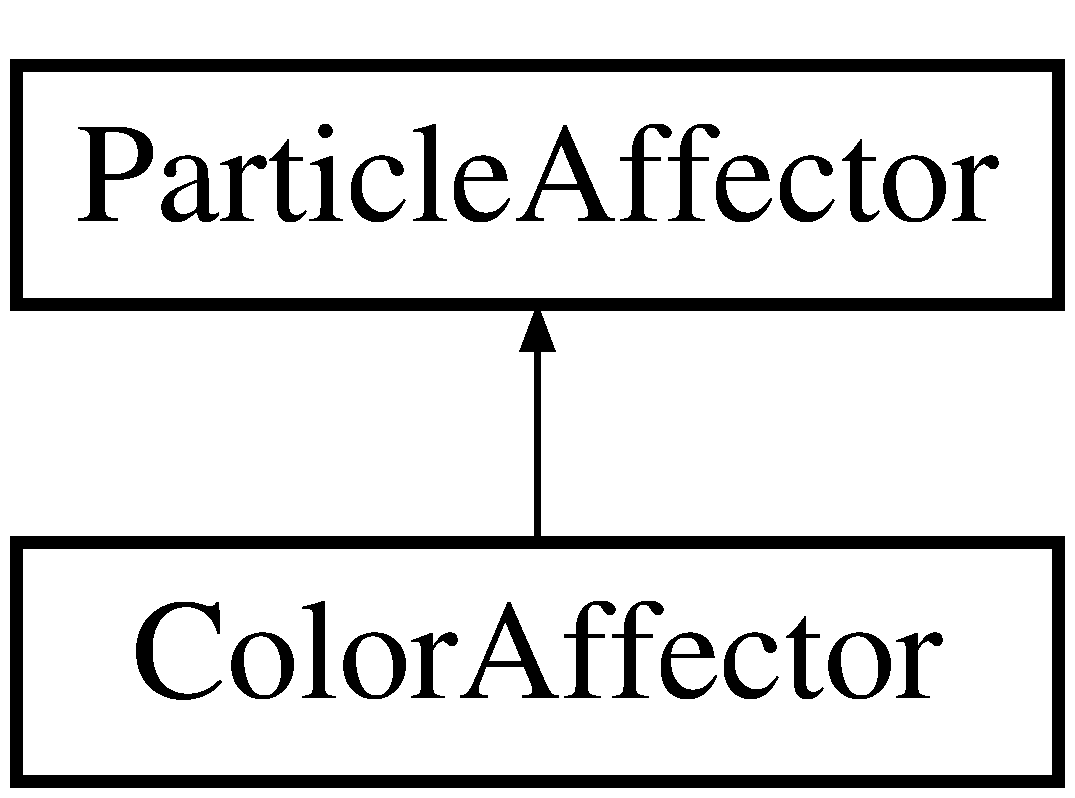
\includegraphics[height=2.000000cm]{class_color_affector}
\end{center}
\end{figure}
\subsection*{Public Member Functions}
\begin{DoxyCompactItemize}
\item 
\mbox{\Hypertarget{class_color_affector_a6e314a66665abd2e74106b8ce4a50180}\label{class_color_affector_a6e314a66665abd2e74106b8ce4a50180}} 
\mbox{\hyperlink{class_color_affector_a6e314a66665abd2e74106b8ce4a50180}{Color\+Affector}} (\mbox{\hyperlink{class_color}{Color}} start\+Color, \mbox{\hyperlink{class_color}{Color}} end\+Color)
\begin{DoxyCompactList}\small\item\em Constructor. start\+Color \+: the color the particle starts with. end\+Color \+: the color the particle would interpolate towards. \end{DoxyCompactList}\item 
\mbox{\Hypertarget{class_color_affector_a9c22679295ea62f47af9f1fe9214b9bc}\label{class_color_affector_a9c22679295ea62f47af9f1fe9214b9bc}} 
virtual void \mbox{\hyperlink{class_color_affector_a9c22679295ea62f47af9f1fe9214b9bc}{affect\+Particle\+Update}} (\mbox{\hyperlink{class_particle_object}{Particle\+Object}} $\ast$particle)
\begin{DoxyCompactList}\small\item\em interpolate the values based on the current life of the particle \end{DoxyCompactList}\end{DoxyCompactItemize}


\subsection{Detailed Description}
Affector that changes particle colors over time. 

The documentation for this class was generated from the following files\+:\begin{DoxyCompactItemize}
\item 
F\+P\+S Counter/Particle\+Affector.\+h\item 
F\+P\+S Counter/Particle\+Affector.\+cpp\end{DoxyCompactItemize}

\hypertarget{struct_color_tree}{}\section{Color\+Tree Struct Reference}
\label{struct_color_tree}\index{Color\+Tree@{Color\+Tree}}
\subsection*{Public Attributes}
\begin{DoxyCompactItemize}
\item 
\mbox{\Hypertarget{struct_color_tree_a46a3b1d9239f5fd467ec97cd067b9a96}\label{struct_color_tree_a46a3b1d9239f5fd467ec97cd067b9a96}} 
\mbox{\hyperlink{struct_color_tree}{Color\+Tree}} $\ast$ {\bfseries children} \mbox{[}16\mbox{]}
\item 
\mbox{\Hypertarget{struct_color_tree_ab3836a4a5981a7cf4ef553d25d9b0361}\label{struct_color_tree_ab3836a4a5981a7cf4ef553d25d9b0361}} 
int {\bfseries index}
\end{DoxyCompactItemize}


The documentation for this struct was generated from the following file\+:\begin{DoxyCompactItemize}
\item 
F\+P\+S Counter/lodepng.\+cpp\end{DoxyCompactItemize}

\hypertarget{class_force_affector}{}\section{Force\+Affector Class Reference}
\label{class_force_affector}\index{Force\+Affector@{Force\+Affector}}


Affector that accelerates particles to a general direction or point.  




{\ttfamily \#include $<$Particle\+Affector.\+h$>$}

Inheritance diagram for Force\+Affector\+:\begin{figure}[H]
\begin{center}
\leavevmode
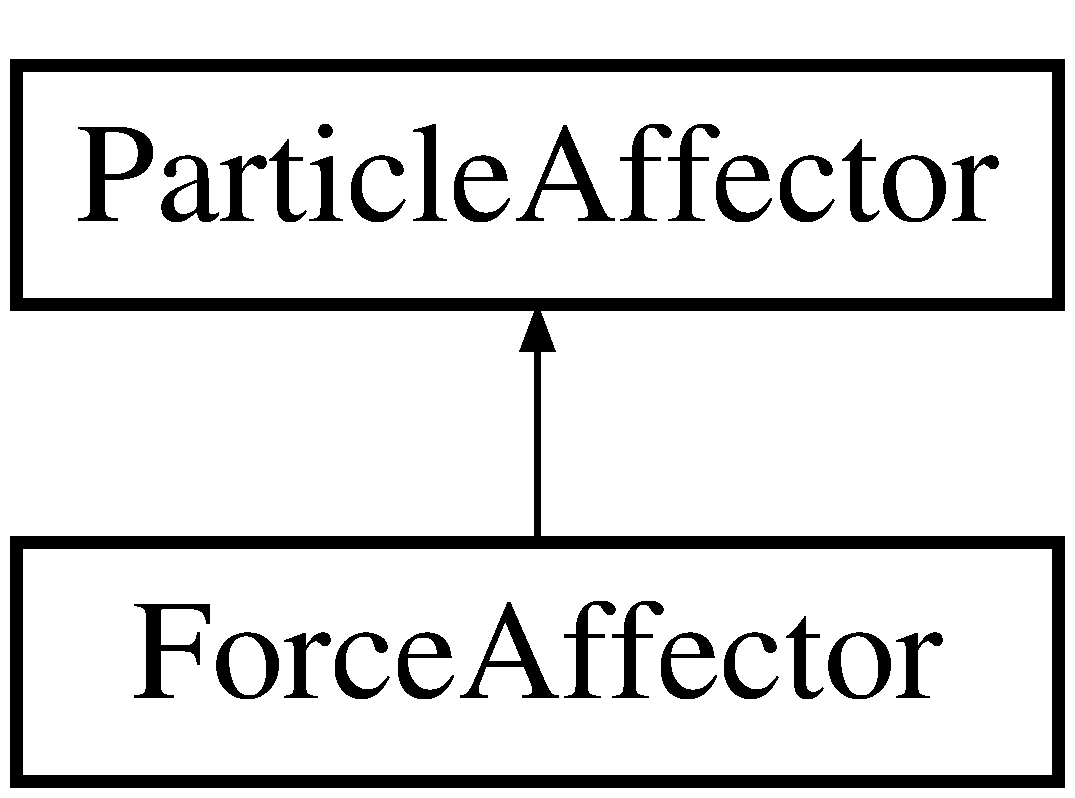
\includegraphics[height=2.000000cm]{class_force_affector}
\end{center}
\end{figure}
\subsection*{Public Member Functions}
\begin{DoxyCompactItemize}
\item 
\mbox{\Hypertarget{class_force_affector_ac644ea9e122d1c890115e0a08d9a0045}\label{class_force_affector_ac644ea9e122d1c890115e0a08d9a0045}} 
\mbox{\hyperlink{class_force_affector_ac644ea9e122d1c890115e0a08d9a0045}{Force\+Affector}} (\mbox{\hyperlink{class_vector3}{Vector3}} direction)
\begin{DoxyCompactList}\small\item\em Constructor. Instantiates a particle system that accelerates the particles to a general direction. Attraction mode \+: G\+E\+N\+E\+R\+AL. \end{DoxyCompactList}\item 
\mbox{\Hypertarget{class_force_affector_adb06c5df310a2f3c903170bd1cb87ea6}\label{class_force_affector_adb06c5df310a2f3c903170bd1cb87ea6}} 
\mbox{\hyperlink{class_force_affector_adb06c5df310a2f3c903170bd1cb87ea6}{Force\+Affector}} (\mbox{\hyperlink{class_vector3}{Vector3}} point, float force)
\begin{DoxyCompactList}\small\item\em Constructor. Instantiates a particle system that accelerates the particles to a point. Attraction mode \+: P\+O\+I\+NT. \end{DoxyCompactList}\item 
\mbox{\Hypertarget{class_force_affector_a3d64d25fb67c854d24b7b714d675477a}\label{class_force_affector_a3d64d25fb67c854d24b7b714d675477a}} 
virtual void \mbox{\hyperlink{class_force_affector_a3d64d25fb67c854d24b7b714d675477a}{affect\+Particle\+Update}} (\mbox{\hyperlink{class_particle_object}{Particle\+Object}} $\ast$particle)
\begin{DoxyCompactList}\small\item\em interpolate the values based on the current life of the particle \end{DoxyCompactList}\end{DoxyCompactItemize}


\subsection{Detailed Description}
Affector that accelerates particles to a general direction or point. 

The documentation for this class was generated from the following files\+:\begin{DoxyCompactItemize}
\item 
F\+P\+S Counter/Particle\+Affector.\+h\item 
F\+P\+S Counter/Particle\+Affector.\+cpp\end{DoxyCompactItemize}

\hypertarget{class_game_object}{}\section{Game\+Object Class Reference}
\label{class_game_object}\index{Game\+Object@{Game\+Object}}
Inheritance diagram for Game\+Object\+:\begin{figure}[H]
\begin{center}
\leavevmode
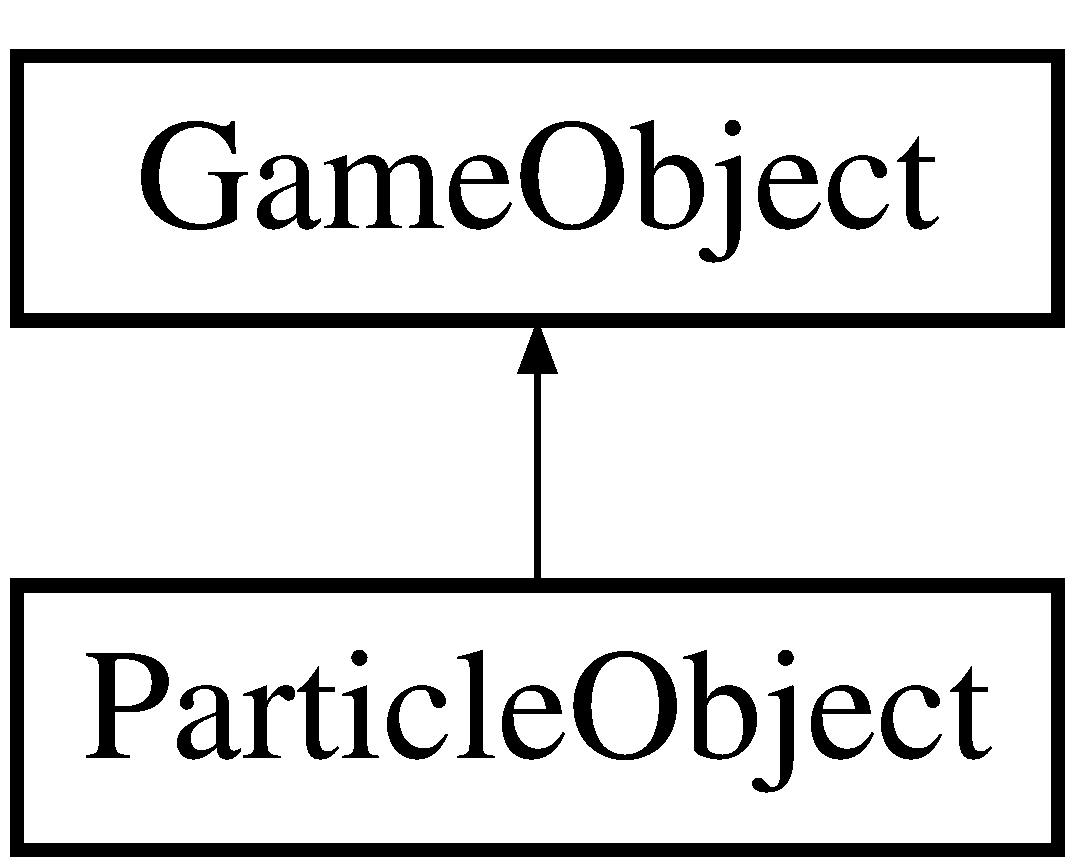
\includegraphics[height=2.000000cm]{class_game_object}
\end{center}
\end{figure}
\subsection*{Public Member Functions}
\begin{DoxyCompactItemize}
\item 
\mbox{\Hypertarget{class_game_object_a8f340c31ff5aa975ae2ed7439fb5d63f}\label{class_game_object_a8f340c31ff5aa975ae2ed7439fb5d63f}} 
{\bfseries Game\+Object} (\mbox{\hyperlink{class_sprite}{Sprite}} $\ast$sprite)
\item 
\mbox{\Hypertarget{class_game_object_a53997902466d2ecb317c4318a3d69816}\label{class_game_object_a53997902466d2ecb317c4318a3d69816}} 
void {\bfseries Set\+Pos} (\mbox{\hyperlink{class_vector3}{Vector3}} pos)
\item 
\mbox{\Hypertarget{class_game_object_ab66324d123ba785d66a11b386a5c0893}\label{class_game_object_ab66324d123ba785d66a11b386a5c0893}} 
const \mbox{\hyperlink{class_vector3}{Vector3}} \& {\bfseries Get\+Pos} ()
\item 
\mbox{\Hypertarget{class_game_object_a82d69d7c9ee269b19cc3528b64281355}\label{class_game_object_a82d69d7c9ee269b19cc3528b64281355}} 
void {\bfseries Set\+Velo\+City} (\mbox{\hyperlink{class_vector3}{Vector3}} velo)
\item 
\mbox{\Hypertarget{class_game_object_a1c0f6935d6ffba2fb08c14f1ee09a6d1}\label{class_game_object_a1c0f6935d6ffba2fb08c14f1ee09a6d1}} 
const \mbox{\hyperlink{class_vector3}{Vector3}} \& {\bfseries Get\+Velocity} ()
\item 
\mbox{\Hypertarget{class_game_object_a58a597b9cd7c9a9e37df1c9d428aa67e}\label{class_game_object_a58a597b9cd7c9a9e37df1c9d428aa67e}} 
void {\bfseries Set\+Rotation} (float rotate)
\item 
\mbox{\Hypertarget{class_game_object_afe8fb5f6303da023e500b1d4b1953b7b}\label{class_game_object_afe8fb5f6303da023e500b1d4b1953b7b}} 
float {\bfseries Get\+Rotation} ()
\item 
\mbox{\Hypertarget{class_game_object_a4ae7e9b3601eb05064f894744aac6074}\label{class_game_object_a4ae7e9b3601eb05064f894744aac6074}} 
void {\bfseries Set\+Scale} (float scale)
\item 
\mbox{\Hypertarget{class_game_object_a513e27cf7361d3c0a9cac3c994cd9017}\label{class_game_object_a513e27cf7361d3c0a9cac3c994cd9017}} 
float {\bfseries Get\+Scale} ()
\item 
\mbox{\Hypertarget{class_game_object_a56f7b1343ae2edad88a1ba9662e76947}\label{class_game_object_a56f7b1343ae2edad88a1ba9662e76947}} 
void {\bfseries Set\+Sprite} (\mbox{\hyperlink{class_sprite}{Sprite}} $\ast$sprite)
\item 
\mbox{\Hypertarget{class_game_object_a58483eb15bd91fc2ec516b1e234cd660}\label{class_game_object_a58483eb15bd91fc2ec516b1e234cd660}} 
\mbox{\hyperlink{class_sprite}{Sprite}} $\ast$ {\bfseries Get\+Sprite} ()
\item 
\mbox{\Hypertarget{class_game_object_a22b28d62e571844384d6d1a5e6eec7a8}\label{class_game_object_a22b28d62e571844384d6d1a5e6eec7a8}} 
void {\bfseries Set\+Color} (const \mbox{\hyperlink{class_color}{Color}} \&color)
\item 
\mbox{\Hypertarget{class_game_object_a0a6f875bbb2657a2a0bed2126a84f0b7}\label{class_game_object_a0a6f875bbb2657a2a0bed2126a84f0b7}} 
const \mbox{\hyperlink{class_color}{Color}} \& {\bfseries Get\+Color} ()
\item 
\mbox{\Hypertarget{class_game_object_a276120a8b680ba3c6e5e8f459c9fc0f4}\label{class_game_object_a276120a8b680ba3c6e5e8f459c9fc0f4}} 
void {\bfseries set\+Blending\+Mode} (enum\+Blend blend)
\item 
\mbox{\Hypertarget{class_game_object_a53e80c55ef5db02d9d70e0487af7464c}\label{class_game_object_a53e80c55ef5db02d9d70e0487af7464c}} 
enum\+Blend {\bfseries get\+Blendingmode} ()
\item 
\mbox{\Hypertarget{class_game_object_abb64143e72358beb808db22182517802}\label{class_game_object_abb64143e72358beb808db22182517802}} 
void {\bfseries draw} ()
\item 
\mbox{\Hypertarget{class_game_object_adad7d284b670db722a2fda8e6a7997e3}\label{class_game_object_adad7d284b670db722a2fda8e6a7997e3}} 
virtual void {\bfseries update} ()
\end{DoxyCompactItemize}
\subsection*{Protected Attributes}
\begin{DoxyCompactItemize}
\item 
\mbox{\Hypertarget{class_game_object_ac117fc8efcc2ccb52e6536c87df8fad1}\label{class_game_object_ac117fc8efcc2ccb52e6536c87df8fad1}} 
\mbox{\hyperlink{class_sprite}{Sprite}} $\ast$ {\bfseries m\+\_\+sprite}
\item 
\mbox{\Hypertarget{class_game_object_acd172f669e9fbea80a388448fb450af5}\label{class_game_object_acd172f669e9fbea80a388448fb450af5}} 
\mbox{\hyperlink{class_vector3}{Vector3}} {\bfseries m\+\_\+position}
\item 
\mbox{\Hypertarget{class_game_object_a86fcd612b3f44c90454fa50e875f73f1}\label{class_game_object_a86fcd612b3f44c90454fa50e875f73f1}} 
\mbox{\hyperlink{class_vector3}{Vector3}} {\bfseries m\+\_\+velocity}
\item 
\mbox{\Hypertarget{class_game_object_a69c4523411c24fd3a4e2b86e748e6742}\label{class_game_object_a69c4523411c24fd3a4e2b86e748e6742}} 
float {\bfseries m\+\_\+rotation}
\item 
\mbox{\Hypertarget{class_game_object_aeacf313d6a432fd7ec7c4197f85a2dc1}\label{class_game_object_aeacf313d6a432fd7ec7c4197f85a2dc1}} 
float {\bfseries m\+\_\+scale}
\item 
\mbox{\Hypertarget{class_game_object_a1771d24fddc27ba4f1940aaaf8a103eb}\label{class_game_object_a1771d24fddc27ba4f1940aaaf8a103eb}} 
\mbox{\hyperlink{class_color}{Color}} {\bfseries m\+\_\+color}
\item 
\mbox{\Hypertarget{class_game_object_aa2167915430a65181290a0b13168bbe1}\label{class_game_object_aa2167915430a65181290a0b13168bbe1}} 
enum\+Blend {\bfseries m\+\_\+blendmode}
\end{DoxyCompactItemize}


The documentation for this class was generated from the following files\+:\begin{DoxyCompactItemize}
\item 
F\+P\+S Counter/Game\+Object.\+h\item 
F\+P\+S Counter/Game\+Object.\+cpp\end{DoxyCompactItemize}

\hypertarget{struct_hash}{}\section{Hash Struct Reference}
\label{struct_hash}\index{Hash@{Hash}}
\subsection*{Public Attributes}
\begin{DoxyCompactItemize}
\item 
\mbox{\Hypertarget{struct_hash_a0977cf12b1d8e6bbc784b5e0877926f5}\label{struct_hash_a0977cf12b1d8e6bbc784b5e0877926f5}} 
int $\ast$ {\bfseries head}
\item 
\mbox{\Hypertarget{struct_hash_abf6ad3db2f652a19cc4ff0792e477899}\label{struct_hash_abf6ad3db2f652a19cc4ff0792e477899}} 
unsigned short $\ast$ {\bfseries chain}
\item 
\mbox{\Hypertarget{struct_hash_a66918968854722efdf7ab5f8ac2c6c1d}\label{struct_hash_a66918968854722efdf7ab5f8ac2c6c1d}} 
int $\ast$ {\bfseries val}
\item 
\mbox{\Hypertarget{struct_hash_a3ed8f51297a858686e11a1a295a3a39c}\label{struct_hash_a3ed8f51297a858686e11a1a295a3a39c}} 
int $\ast$ {\bfseries headz}
\item 
\mbox{\Hypertarget{struct_hash_a04ef237e7bc2fa99bc7305fb2352084d}\label{struct_hash_a04ef237e7bc2fa99bc7305fb2352084d}} 
unsigned short $\ast$ {\bfseries chainz}
\item 
\mbox{\Hypertarget{struct_hash_a7247caa3e23eaba8f0d199ec5010c931}\label{struct_hash_a7247caa3e23eaba8f0d199ec5010c931}} 
unsigned short $\ast$ {\bfseries zeros}
\end{DoxyCompactItemize}


The documentation for this struct was generated from the following file\+:\begin{DoxyCompactItemize}
\item 
F\+P\+S Counter/lodepng.\+cpp\end{DoxyCompactItemize}

\hypertarget{struct_huffman_tree}{}\section{Huffman\+Tree Struct Reference}
\label{struct_huffman_tree}\index{Huffman\+Tree@{Huffman\+Tree}}
\subsection*{Public Attributes}
\begin{DoxyCompactItemize}
\item 
\mbox{\Hypertarget{struct_huffman_tree_a91160304cb771d2f9f39ee357c9b05a8}\label{struct_huffman_tree_a91160304cb771d2f9f39ee357c9b05a8}} 
unsigned $\ast$ {\bfseries tree2d}
\item 
\mbox{\Hypertarget{struct_huffman_tree_a47b3346a25fe0a3222b595c236ad146e}\label{struct_huffman_tree_a47b3346a25fe0a3222b595c236ad146e}} 
unsigned $\ast$ {\bfseries tree1d}
\item 
\mbox{\Hypertarget{struct_huffman_tree_aef81d45a5c56276c5699a8e9a575021d}\label{struct_huffman_tree_aef81d45a5c56276c5699a8e9a575021d}} 
unsigned $\ast$ {\bfseries lengths}
\item 
\mbox{\Hypertarget{struct_huffman_tree_adf034ca9ce62a4ebfffaaeaba4378a26}\label{struct_huffman_tree_adf034ca9ce62a4ebfffaaeaba4378a26}} 
unsigned {\bfseries maxbitlen}
\item 
\mbox{\Hypertarget{struct_huffman_tree_a608df5a24f60d1077a5cde19d5149e1f}\label{struct_huffman_tree_a608df5a24f60d1077a5cde19d5149e1f}} 
unsigned {\bfseries numcodes}
\end{DoxyCompactItemize}


The documentation for this struct was generated from the following file\+:\begin{DoxyCompactItemize}
\item 
F\+P\+S Counter/lodepng.\+cpp\end{DoxyCompactItemize}

\hypertarget{struct_lode_p_n_g_color_mode}{}\section{Lode\+P\+N\+G\+Color\+Mode Struct Reference}
\label{struct_lode_p_n_g_color_mode}\index{Lode\+P\+N\+G\+Color\+Mode@{Lode\+P\+N\+G\+Color\+Mode}}
\subsection*{Public Attributes}
\begin{DoxyCompactItemize}
\item 
\mbox{\Hypertarget{struct_lode_p_n_g_color_mode_a4f3df7240411abe80546052d197fbe8d}\label{struct_lode_p_n_g_color_mode_a4f3df7240411abe80546052d197fbe8d}} 
Lode\+P\+N\+G\+Color\+Type {\bfseries colortype}
\item 
\mbox{\Hypertarget{struct_lode_p_n_g_color_mode_ad20010b9561980f65281bc17f7848253}\label{struct_lode_p_n_g_color_mode_ad20010b9561980f65281bc17f7848253}} 
unsigned {\bfseries bitdepth}
\item 
\mbox{\Hypertarget{struct_lode_p_n_g_color_mode_a54f0a793238009fcb95f081626fae308}\label{struct_lode_p_n_g_color_mode_a54f0a793238009fcb95f081626fae308}} 
unsigned char $\ast$ {\bfseries palette}
\item 
\mbox{\Hypertarget{struct_lode_p_n_g_color_mode_a407557f056168682d9319aeb60866dcc}\label{struct_lode_p_n_g_color_mode_a407557f056168682d9319aeb60866dcc}} 
size\+\_\+t {\bfseries palettesize}
\item 
\mbox{\Hypertarget{struct_lode_p_n_g_color_mode_ab9105505c5d56cfc6ce4efe1bb288b54}\label{struct_lode_p_n_g_color_mode_ab9105505c5d56cfc6ce4efe1bb288b54}} 
unsigned {\bfseries key\+\_\+defined}
\item 
\mbox{\Hypertarget{struct_lode_p_n_g_color_mode_a29e64327bca1f3d16235e9ff471e4d50}\label{struct_lode_p_n_g_color_mode_a29e64327bca1f3d16235e9ff471e4d50}} 
unsigned {\bfseries key\+\_\+r}
\item 
\mbox{\Hypertarget{struct_lode_p_n_g_color_mode_ad98309f36d289392b0c440baa50af9f6}\label{struct_lode_p_n_g_color_mode_ad98309f36d289392b0c440baa50af9f6}} 
unsigned {\bfseries key\+\_\+g}
\item 
\mbox{\Hypertarget{struct_lode_p_n_g_color_mode_a93a269405fee0d1c5045a1a671ed1de8}\label{struct_lode_p_n_g_color_mode_a93a269405fee0d1c5045a1a671ed1de8}} 
unsigned {\bfseries key\+\_\+b}
\end{DoxyCompactItemize}


The documentation for this struct was generated from the following file\+:\begin{DoxyCompactItemize}
\item 
F\+P\+S Counter/lodepng.\+h\end{DoxyCompactItemize}

\hypertarget{struct_lode_p_n_g_color_profile}{}\section{Lode\+P\+N\+G\+Color\+Profile Struct Reference}
\label{struct_lode_p_n_g_color_profile}\index{Lode\+P\+N\+G\+Color\+Profile@{Lode\+P\+N\+G\+Color\+Profile}}
\subsection*{Public Attributes}
\begin{DoxyCompactItemize}
\item 
\mbox{\Hypertarget{struct_lode_p_n_g_color_profile_abf063a566a4ab9f4d71b49764573d610}\label{struct_lode_p_n_g_color_profile_abf063a566a4ab9f4d71b49764573d610}} 
unsigned {\bfseries colored}
\item 
\mbox{\Hypertarget{struct_lode_p_n_g_color_profile_a24f19f400a53672340877eefbc837b0c}\label{struct_lode_p_n_g_color_profile_a24f19f400a53672340877eefbc837b0c}} 
unsigned {\bfseries key}
\item 
\mbox{\Hypertarget{struct_lode_p_n_g_color_profile_a0398985ae0572ef97e83c33c7486cafd}\label{struct_lode_p_n_g_color_profile_a0398985ae0572ef97e83c33c7486cafd}} 
unsigned short {\bfseries key\+\_\+r}
\item 
\mbox{\Hypertarget{struct_lode_p_n_g_color_profile_aba03e973374bd15315b8c01b86e94e8f}\label{struct_lode_p_n_g_color_profile_aba03e973374bd15315b8c01b86e94e8f}} 
unsigned short {\bfseries key\+\_\+g}
\item 
\mbox{\Hypertarget{struct_lode_p_n_g_color_profile_a39b65ec69f6aaee3ee7312a993f21e40}\label{struct_lode_p_n_g_color_profile_a39b65ec69f6aaee3ee7312a993f21e40}} 
unsigned short {\bfseries key\+\_\+b}
\item 
\mbox{\Hypertarget{struct_lode_p_n_g_color_profile_a554fea329af8034e91e1cdd8c1af0d90}\label{struct_lode_p_n_g_color_profile_a554fea329af8034e91e1cdd8c1af0d90}} 
unsigned {\bfseries alpha}
\item 
\mbox{\Hypertarget{struct_lode_p_n_g_color_profile_afdce0f5fbec46d6b8f1ec63da0a285f9}\label{struct_lode_p_n_g_color_profile_afdce0f5fbec46d6b8f1ec63da0a285f9}} 
unsigned {\bfseries numcolors}
\item 
\mbox{\Hypertarget{struct_lode_p_n_g_color_profile_a223f8bee4c9ae8be0b70cc08f19aaead}\label{struct_lode_p_n_g_color_profile_a223f8bee4c9ae8be0b70cc08f19aaead}} 
unsigned char {\bfseries palette} \mbox{[}1024\mbox{]}
\item 
\mbox{\Hypertarget{struct_lode_p_n_g_color_profile_a1d3870b03dfe6d699bf4c968c9bc1890}\label{struct_lode_p_n_g_color_profile_a1d3870b03dfe6d699bf4c968c9bc1890}} 
unsigned {\bfseries bits}
\end{DoxyCompactItemize}


The documentation for this struct was generated from the following file\+:\begin{DoxyCompactItemize}
\item 
F\+P\+S Counter/lodepng.\+h\end{DoxyCompactItemize}

\hypertarget{struct_lode_p_n_g_compress_settings}{}\section{Lode\+P\+N\+G\+Compress\+Settings Struct Reference}
\label{struct_lode_p_n_g_compress_settings}\index{Lode\+P\+N\+G\+Compress\+Settings@{Lode\+P\+N\+G\+Compress\+Settings}}
\subsection*{Public Attributes}
\begin{DoxyCompactItemize}
\item 
\mbox{\Hypertarget{struct_lode_p_n_g_compress_settings_ac0afeac7276cce01fa9824aa2d5a1ba9}\label{struct_lode_p_n_g_compress_settings_ac0afeac7276cce01fa9824aa2d5a1ba9}} 
unsigned {\bfseries btype}
\item 
\mbox{\Hypertarget{struct_lode_p_n_g_compress_settings_a37a87bd874376f0298efad2870e70e7e}\label{struct_lode_p_n_g_compress_settings_a37a87bd874376f0298efad2870e70e7e}} 
unsigned {\bfseries use\+\_\+lz77}
\item 
\mbox{\Hypertarget{struct_lode_p_n_g_compress_settings_a01e77a9db5c2c4dfe6c79bf04f0bf84e}\label{struct_lode_p_n_g_compress_settings_a01e77a9db5c2c4dfe6c79bf04f0bf84e}} 
unsigned {\bfseries windowsize}
\item 
\mbox{\Hypertarget{struct_lode_p_n_g_compress_settings_a11d89e0ff0c57f1c49dd58cb8347e005}\label{struct_lode_p_n_g_compress_settings_a11d89e0ff0c57f1c49dd58cb8347e005}} 
unsigned {\bfseries minmatch}
\item 
\mbox{\Hypertarget{struct_lode_p_n_g_compress_settings_a70bc37e21eeffead6e9c8d67e163a591}\label{struct_lode_p_n_g_compress_settings_a70bc37e21eeffead6e9c8d67e163a591}} 
unsigned {\bfseries nicematch}
\item 
\mbox{\Hypertarget{struct_lode_p_n_g_compress_settings_ad4ffde429dee40a8c314016f5f6fdab5}\label{struct_lode_p_n_g_compress_settings_ad4ffde429dee40a8c314016f5f6fdab5}} 
unsigned {\bfseries lazymatching}
\item 
\mbox{\Hypertarget{struct_lode_p_n_g_compress_settings_a4a7835f394349f15f1302d11bcb0efa0}\label{struct_lode_p_n_g_compress_settings_a4a7835f394349f15f1302d11bcb0efa0}} 
unsigned($\ast$ {\bfseries custom\+\_\+zlib} )(unsigned char $\ast$$\ast$, size\+\_\+t $\ast$, const unsigned char $\ast$, size\+\_\+t, const \mbox{\hyperlink{struct_lode_p_n_g_compress_settings}{Lode\+P\+N\+G\+Compress\+Settings}} $\ast$)
\item 
\mbox{\Hypertarget{struct_lode_p_n_g_compress_settings_a55dafebbbe017806fb2bbc32bb40a59b}\label{struct_lode_p_n_g_compress_settings_a55dafebbbe017806fb2bbc32bb40a59b}} 
unsigned($\ast$ {\bfseries custom\+\_\+deflate} )(unsigned char $\ast$$\ast$, size\+\_\+t $\ast$, const unsigned char $\ast$, size\+\_\+t, const \mbox{\hyperlink{struct_lode_p_n_g_compress_settings}{Lode\+P\+N\+G\+Compress\+Settings}} $\ast$)
\item 
\mbox{\Hypertarget{struct_lode_p_n_g_compress_settings_a62826645ef28e2a84dd2b65f547a2883}\label{struct_lode_p_n_g_compress_settings_a62826645ef28e2a84dd2b65f547a2883}} 
const void $\ast$ {\bfseries custom\+\_\+context}
\end{DoxyCompactItemize}


The documentation for this struct was generated from the following file\+:\begin{DoxyCompactItemize}
\item 
F\+P\+S Counter/lodepng.\+h\end{DoxyCompactItemize}

\hypertarget{struct_lode_p_n_g_decoder_settings}{}\section{Lode\+P\+N\+G\+Decoder\+Settings Struct Reference}
\label{struct_lode_p_n_g_decoder_settings}\index{Lode\+P\+N\+G\+Decoder\+Settings@{Lode\+P\+N\+G\+Decoder\+Settings}}
\subsection*{Public Attributes}
\begin{DoxyCompactItemize}
\item 
\mbox{\Hypertarget{struct_lode_p_n_g_decoder_settings_a9ae8fef9880bef97a3e932f8ea942ed8}\label{struct_lode_p_n_g_decoder_settings_a9ae8fef9880bef97a3e932f8ea942ed8}} 
\mbox{\hyperlink{struct_lode_p_n_g_decompress_settings}{Lode\+P\+N\+G\+Decompress\+Settings}} {\bfseries zlibsettings}
\item 
\mbox{\Hypertarget{struct_lode_p_n_g_decoder_settings_a6390c403d2a5718242337bbbaf15131d}\label{struct_lode_p_n_g_decoder_settings_a6390c403d2a5718242337bbbaf15131d}} 
unsigned {\bfseries ignore\+\_\+crc}
\item 
\mbox{\Hypertarget{struct_lode_p_n_g_decoder_settings_af26f2b29cd338ce4476bee9571a0818a}\label{struct_lode_p_n_g_decoder_settings_af26f2b29cd338ce4476bee9571a0818a}} 
unsigned {\bfseries color\+\_\+convert}
\item 
\mbox{\Hypertarget{struct_lode_p_n_g_decoder_settings_aa1212905c3f73d9fffef2c04a220d951}\label{struct_lode_p_n_g_decoder_settings_aa1212905c3f73d9fffef2c04a220d951}} 
unsigned {\bfseries read\+\_\+text\+\_\+chunks}
\item 
\mbox{\Hypertarget{struct_lode_p_n_g_decoder_settings_a8775e4fc539dc457916720f52b442f27}\label{struct_lode_p_n_g_decoder_settings_a8775e4fc539dc457916720f52b442f27}} 
unsigned {\bfseries remember\+\_\+unknown\+\_\+chunks}
\end{DoxyCompactItemize}


The documentation for this struct was generated from the following file\+:\begin{DoxyCompactItemize}
\item 
F\+P\+S Counter/lodepng.\+h\end{DoxyCompactItemize}

\hypertarget{struct_lode_p_n_g_decompress_settings}{}\section{Lode\+P\+N\+G\+Decompress\+Settings Struct Reference}
\label{struct_lode_p_n_g_decompress_settings}\index{Lode\+P\+N\+G\+Decompress\+Settings@{Lode\+P\+N\+G\+Decompress\+Settings}}
\subsection*{Public Attributes}
\begin{DoxyCompactItemize}
\item 
\mbox{\Hypertarget{struct_lode_p_n_g_decompress_settings_afab4b919650b51b4d2f175a60ed6c580}\label{struct_lode_p_n_g_decompress_settings_afab4b919650b51b4d2f175a60ed6c580}} 
unsigned {\bfseries ignore\+\_\+adler32}
\item 
\mbox{\Hypertarget{struct_lode_p_n_g_decompress_settings_a9dd432e46330dbd2ce3ef1929c64337d}\label{struct_lode_p_n_g_decompress_settings_a9dd432e46330dbd2ce3ef1929c64337d}} 
unsigned($\ast$ {\bfseries custom\+\_\+zlib} )(unsigned char $\ast$$\ast$, size\+\_\+t $\ast$, const unsigned char $\ast$, size\+\_\+t, const \mbox{\hyperlink{struct_lode_p_n_g_decompress_settings}{Lode\+P\+N\+G\+Decompress\+Settings}} $\ast$)
\item 
\mbox{\Hypertarget{struct_lode_p_n_g_decompress_settings_a023aa5946c99934d40280850a4d8b204}\label{struct_lode_p_n_g_decompress_settings_a023aa5946c99934d40280850a4d8b204}} 
unsigned($\ast$ {\bfseries custom\+\_\+inflate} )(unsigned char $\ast$$\ast$, size\+\_\+t $\ast$, const unsigned char $\ast$, size\+\_\+t, const \mbox{\hyperlink{struct_lode_p_n_g_decompress_settings}{Lode\+P\+N\+G\+Decompress\+Settings}} $\ast$)
\item 
\mbox{\Hypertarget{struct_lode_p_n_g_decompress_settings_a66e3608b541c64bb275c0ac1a80c3ec6}\label{struct_lode_p_n_g_decompress_settings_a66e3608b541c64bb275c0ac1a80c3ec6}} 
const void $\ast$ {\bfseries custom\+\_\+context}
\end{DoxyCompactItemize}


The documentation for this struct was generated from the following file\+:\begin{DoxyCompactItemize}
\item 
F\+P\+S Counter/lodepng.\+h\end{DoxyCompactItemize}

\hypertarget{struct_lode_p_n_g_encoder_settings}{}\section{Lode\+P\+N\+G\+Encoder\+Settings Struct Reference}
\label{struct_lode_p_n_g_encoder_settings}\index{Lode\+P\+N\+G\+Encoder\+Settings@{Lode\+P\+N\+G\+Encoder\+Settings}}
\subsection*{Public Attributes}
\begin{DoxyCompactItemize}
\item 
\mbox{\Hypertarget{struct_lode_p_n_g_encoder_settings_a2c5928b4172c75e27de467870f2ff946}\label{struct_lode_p_n_g_encoder_settings_a2c5928b4172c75e27de467870f2ff946}} 
\mbox{\hyperlink{struct_lode_p_n_g_compress_settings}{Lode\+P\+N\+G\+Compress\+Settings}} {\bfseries zlibsettings}
\item 
\mbox{\Hypertarget{struct_lode_p_n_g_encoder_settings_a1203b8db6532c9ff4a5c8ee692cd327a}\label{struct_lode_p_n_g_encoder_settings_a1203b8db6532c9ff4a5c8ee692cd327a}} 
unsigned {\bfseries auto\+\_\+convert}
\item 
\mbox{\Hypertarget{struct_lode_p_n_g_encoder_settings_a0d82e8f2fabcb6cebbc54b80922945f1}\label{struct_lode_p_n_g_encoder_settings_a0d82e8f2fabcb6cebbc54b80922945f1}} 
unsigned {\bfseries filter\+\_\+palette\+\_\+zero}
\item 
\mbox{\Hypertarget{struct_lode_p_n_g_encoder_settings_a5e18e4eb941763a2e3e6c65ee9f0729c}\label{struct_lode_p_n_g_encoder_settings_a5e18e4eb941763a2e3e6c65ee9f0729c}} 
Lode\+P\+N\+G\+Filter\+Strategy {\bfseries filter\+\_\+strategy}
\item 
\mbox{\Hypertarget{struct_lode_p_n_g_encoder_settings_a4446f87b5283f25664802a1be037e76e}\label{struct_lode_p_n_g_encoder_settings_a4446f87b5283f25664802a1be037e76e}} 
const unsigned char $\ast$ {\bfseries predefined\+\_\+filters}
\item 
\mbox{\Hypertarget{struct_lode_p_n_g_encoder_settings_a04dc9622ccd1d7c74c56291409aa512a}\label{struct_lode_p_n_g_encoder_settings_a04dc9622ccd1d7c74c56291409aa512a}} 
unsigned {\bfseries force\+\_\+palette}
\item 
\mbox{\Hypertarget{struct_lode_p_n_g_encoder_settings_a893aa542aa7c122c32ee36dd716fbcb2}\label{struct_lode_p_n_g_encoder_settings_a893aa542aa7c122c32ee36dd716fbcb2}} 
unsigned {\bfseries add\+\_\+id}
\item 
\mbox{\Hypertarget{struct_lode_p_n_g_encoder_settings_a6ffdcb8e85a65ea208fe027be072d710}\label{struct_lode_p_n_g_encoder_settings_a6ffdcb8e85a65ea208fe027be072d710}} 
unsigned {\bfseries text\+\_\+compression}
\end{DoxyCompactItemize}


The documentation for this struct was generated from the following file\+:\begin{DoxyCompactItemize}
\item 
F\+P\+S Counter/lodepng.\+h\end{DoxyCompactItemize}

\hypertarget{struct_lode_p_n_g_info}{}\section{Lode\+P\+N\+G\+Info Struct Reference}
\label{struct_lode_p_n_g_info}\index{Lode\+P\+N\+G\+Info@{Lode\+P\+N\+G\+Info}}
\subsection*{Public Attributes}
\begin{DoxyCompactItemize}
\item 
\mbox{\Hypertarget{struct_lode_p_n_g_info_a42bcacd0dbaaea01c04cc87b58ac3c1d}\label{struct_lode_p_n_g_info_a42bcacd0dbaaea01c04cc87b58ac3c1d}} 
unsigned {\bfseries compression\+\_\+method}
\item 
\mbox{\Hypertarget{struct_lode_p_n_g_info_a5098d6e8aa528d5197f51914439633b9}\label{struct_lode_p_n_g_info_a5098d6e8aa528d5197f51914439633b9}} 
unsigned {\bfseries filter\+\_\+method}
\item 
\mbox{\Hypertarget{struct_lode_p_n_g_info_a80207e3e53c959b2285636496a3dd3f1}\label{struct_lode_p_n_g_info_a80207e3e53c959b2285636496a3dd3f1}} 
unsigned {\bfseries interlace\+\_\+method}
\item 
\mbox{\Hypertarget{struct_lode_p_n_g_info_a0af9bab3435084780ce8c1cb69bb2628}\label{struct_lode_p_n_g_info_a0af9bab3435084780ce8c1cb69bb2628}} 
\mbox{\hyperlink{struct_lode_p_n_g_color_mode}{Lode\+P\+N\+G\+Color\+Mode}} {\bfseries color}
\item 
\mbox{\Hypertarget{struct_lode_p_n_g_info_aa94c65344af02472adb9c71eae2e765f}\label{struct_lode_p_n_g_info_aa94c65344af02472adb9c71eae2e765f}} 
unsigned {\bfseries background\+\_\+defined}
\item 
\mbox{\Hypertarget{struct_lode_p_n_g_info_a98b59c3760bda184bb16c9713b430bc3}\label{struct_lode_p_n_g_info_a98b59c3760bda184bb16c9713b430bc3}} 
unsigned {\bfseries background\+\_\+r}
\item 
\mbox{\Hypertarget{struct_lode_p_n_g_info_abf638e191edaeaa2b02c371a381e3a89}\label{struct_lode_p_n_g_info_abf638e191edaeaa2b02c371a381e3a89}} 
unsigned {\bfseries background\+\_\+g}
\item 
\mbox{\Hypertarget{struct_lode_p_n_g_info_a994de0c74ef1092f056ff534e00dfa0d}\label{struct_lode_p_n_g_info_a994de0c74ef1092f056ff534e00dfa0d}} 
unsigned {\bfseries background\+\_\+b}
\item 
\mbox{\Hypertarget{struct_lode_p_n_g_info_a393e0b3948ca6674232e1cc625db282e}\label{struct_lode_p_n_g_info_a393e0b3948ca6674232e1cc625db282e}} 
size\+\_\+t {\bfseries text\+\_\+num}
\item 
\mbox{\Hypertarget{struct_lode_p_n_g_info_a0a26147c9673870dd122693f17a69b13}\label{struct_lode_p_n_g_info_a0a26147c9673870dd122693f17a69b13}} 
char $\ast$$\ast$ {\bfseries text\+\_\+keys}
\item 
\mbox{\Hypertarget{struct_lode_p_n_g_info_aac321d27e65c54e56d6092d3a6400a81}\label{struct_lode_p_n_g_info_aac321d27e65c54e56d6092d3a6400a81}} 
char $\ast$$\ast$ {\bfseries text\+\_\+strings}
\item 
\mbox{\Hypertarget{struct_lode_p_n_g_info_a22166bb10c89a4d80e206d6c4736b625}\label{struct_lode_p_n_g_info_a22166bb10c89a4d80e206d6c4736b625}} 
size\+\_\+t {\bfseries itext\+\_\+num}
\item 
\mbox{\Hypertarget{struct_lode_p_n_g_info_a1b909e03596abf86d564641741b0087f}\label{struct_lode_p_n_g_info_a1b909e03596abf86d564641741b0087f}} 
char $\ast$$\ast$ {\bfseries itext\+\_\+keys}
\item 
\mbox{\Hypertarget{struct_lode_p_n_g_info_ae9f9f594e63c910d467a14f550960837}\label{struct_lode_p_n_g_info_ae9f9f594e63c910d467a14f550960837}} 
char $\ast$$\ast$ {\bfseries itext\+\_\+langtags}
\item 
\mbox{\Hypertarget{struct_lode_p_n_g_info_a93a8e823ac715dbdd625f023d8fdebc2}\label{struct_lode_p_n_g_info_a93a8e823ac715dbdd625f023d8fdebc2}} 
char $\ast$$\ast$ {\bfseries itext\+\_\+transkeys}
\item 
\mbox{\Hypertarget{struct_lode_p_n_g_info_a7014fd40ffeb1d482f72d33c020cf73e}\label{struct_lode_p_n_g_info_a7014fd40ffeb1d482f72d33c020cf73e}} 
char $\ast$$\ast$ {\bfseries itext\+\_\+strings}
\item 
\mbox{\Hypertarget{struct_lode_p_n_g_info_a9adb9f74ab90716ae107b99da5384424}\label{struct_lode_p_n_g_info_a9adb9f74ab90716ae107b99da5384424}} 
unsigned {\bfseries time\+\_\+defined}
\item 
\mbox{\Hypertarget{struct_lode_p_n_g_info_a4d3407acdf79bf87f20a3562f210b393}\label{struct_lode_p_n_g_info_a4d3407acdf79bf87f20a3562f210b393}} 
\mbox{\hyperlink{struct_lode_p_n_g_time}{Lode\+P\+N\+G\+Time}} {\bfseries time}
\item 
\mbox{\Hypertarget{struct_lode_p_n_g_info_a9b8e29b7e7b4908a2de0275e01a828ed}\label{struct_lode_p_n_g_info_a9b8e29b7e7b4908a2de0275e01a828ed}} 
unsigned {\bfseries phys\+\_\+defined}
\item 
\mbox{\Hypertarget{struct_lode_p_n_g_info_a1593fa6e1acc93f3b9de51c340bef94d}\label{struct_lode_p_n_g_info_a1593fa6e1acc93f3b9de51c340bef94d}} 
unsigned {\bfseries phys\+\_\+x}
\item 
\mbox{\Hypertarget{struct_lode_p_n_g_info_a52ad7a105244d00f1e91c489eaf53f97}\label{struct_lode_p_n_g_info_a52ad7a105244d00f1e91c489eaf53f97}} 
unsigned {\bfseries phys\+\_\+y}
\item 
\mbox{\Hypertarget{struct_lode_p_n_g_info_ad6f2171d9f87716e5010f6c5352f9855}\label{struct_lode_p_n_g_info_ad6f2171d9f87716e5010f6c5352f9855}} 
unsigned {\bfseries phys\+\_\+unit}
\item 
\mbox{\Hypertarget{struct_lode_p_n_g_info_a8347476da7fc2fc6af4ec7ed44b638c6}\label{struct_lode_p_n_g_info_a8347476da7fc2fc6af4ec7ed44b638c6}} 
unsigned char $\ast$ {\bfseries unknown\+\_\+chunks\+\_\+data} \mbox{[}3\mbox{]}
\item 
\mbox{\Hypertarget{struct_lode_p_n_g_info_a25a81d760759bd0383ae5a81ba83911d}\label{struct_lode_p_n_g_info_a25a81d760759bd0383ae5a81ba83911d}} 
size\+\_\+t {\bfseries unknown\+\_\+chunks\+\_\+size} \mbox{[}3\mbox{]}
\end{DoxyCompactItemize}


The documentation for this struct was generated from the following file\+:\begin{DoxyCompactItemize}
\item 
F\+P\+S Counter/lodepng.\+h\end{DoxyCompactItemize}

\hypertarget{struct_lode_p_n_g_state}{}\section{Lode\+P\+N\+G\+State Struct Reference}
\label{struct_lode_p_n_g_state}\index{Lode\+P\+N\+G\+State@{Lode\+P\+N\+G\+State}}
\subsection*{Public Attributes}
\begin{DoxyCompactItemize}
\item 
\mbox{\Hypertarget{struct_lode_p_n_g_state_abd2c38ffc68f04b0e4159e1f97ba1f76}\label{struct_lode_p_n_g_state_abd2c38ffc68f04b0e4159e1f97ba1f76}} 
\mbox{\hyperlink{struct_lode_p_n_g_decoder_settings}{Lode\+P\+N\+G\+Decoder\+Settings}} {\bfseries decoder}
\item 
\mbox{\Hypertarget{struct_lode_p_n_g_state_ac63d91db835129d02eb83bbe81de347e}\label{struct_lode_p_n_g_state_ac63d91db835129d02eb83bbe81de347e}} 
\mbox{\hyperlink{struct_lode_p_n_g_encoder_settings}{Lode\+P\+N\+G\+Encoder\+Settings}} {\bfseries encoder}
\item 
\mbox{\Hypertarget{struct_lode_p_n_g_state_a597bc08de787147474d43adf8b6ceacf}\label{struct_lode_p_n_g_state_a597bc08de787147474d43adf8b6ceacf}} 
\mbox{\hyperlink{struct_lode_p_n_g_color_mode}{Lode\+P\+N\+G\+Color\+Mode}} {\bfseries info\+\_\+raw}
\item 
\mbox{\Hypertarget{struct_lode_p_n_g_state_a08d9ac43c995fcf34d72b1d37047b6fa}\label{struct_lode_p_n_g_state_a08d9ac43c995fcf34d72b1d37047b6fa}} 
\mbox{\hyperlink{struct_lode_p_n_g_info}{Lode\+P\+N\+G\+Info}} {\bfseries info\+\_\+png}
\item 
\mbox{\Hypertarget{struct_lode_p_n_g_state_a1a00a050da588cf3c2b7a6252bebb0cd}\label{struct_lode_p_n_g_state_a1a00a050da588cf3c2b7a6252bebb0cd}} 
unsigned {\bfseries error}
\end{DoxyCompactItemize}


The documentation for this struct was generated from the following file\+:\begin{DoxyCompactItemize}
\item 
F\+P\+S Counter/lodepng.\+h\end{DoxyCompactItemize}

\hypertarget{struct_lode_p_n_g_time}{}\section{Lode\+P\+N\+G\+Time Struct Reference}
\label{struct_lode_p_n_g_time}\index{Lode\+P\+N\+G\+Time@{Lode\+P\+N\+G\+Time}}
\subsection*{Public Attributes}
\begin{DoxyCompactItemize}
\item 
\mbox{\Hypertarget{struct_lode_p_n_g_time_a32b68342f39f3d38ba91a721b1149b8f}\label{struct_lode_p_n_g_time_a32b68342f39f3d38ba91a721b1149b8f}} 
unsigned {\bfseries year}
\item 
\mbox{\Hypertarget{struct_lode_p_n_g_time_a295d890e862d5cd0c444e9d3a96fa9d5}\label{struct_lode_p_n_g_time_a295d890e862d5cd0c444e9d3a96fa9d5}} 
unsigned {\bfseries month}
\item 
\mbox{\Hypertarget{struct_lode_p_n_g_time_aa3dee3b7b3a1e730fbded7a7b8cf355e}\label{struct_lode_p_n_g_time_aa3dee3b7b3a1e730fbded7a7b8cf355e}} 
unsigned {\bfseries day}
\item 
\mbox{\Hypertarget{struct_lode_p_n_g_time_ac99cb7f3ce16a85f9f505b7f5f6e0aa7}\label{struct_lode_p_n_g_time_ac99cb7f3ce16a85f9f505b7f5f6e0aa7}} 
unsigned {\bfseries hour}
\item 
\mbox{\Hypertarget{struct_lode_p_n_g_time_ac3045de79728f29fc61f534b062e0f13}\label{struct_lode_p_n_g_time_ac3045de79728f29fc61f534b062e0f13}} 
unsigned {\bfseries minute}
\item 
\mbox{\Hypertarget{struct_lode_p_n_g_time_a6c691c5821e828488a8bb8a90751a2f0}\label{struct_lode_p_n_g_time_a6c691c5821e828488a8bb8a90751a2f0}} 
unsigned {\bfseries second}
\end{DoxyCompactItemize}


The documentation for this struct was generated from the following file\+:\begin{DoxyCompactItemize}
\item 
F\+P\+S Counter/lodepng.\+h\end{DoxyCompactItemize}

\hypertarget{class_matrix}{}\section{Matrix Class Reference}
\label{class_matrix}\index{Matrix@{Matrix}}
\subsection*{Public Member Functions}
\begin{DoxyCompactItemize}
\item 
\mbox{\Hypertarget{class_matrix_a2dba13c45127354c9f75ef576f49269b}\label{class_matrix_a2dba13c45127354c9f75ef576f49269b}} 
\mbox{\hyperlink{class_matrix_a2dba13c45127354c9f75ef576f49269b}{Matrix}} ()
\begin{DoxyCompactList}\small\item\em Constructor. \end{DoxyCompactList}\item 
\mbox{\Hypertarget{class_matrix_abcf708e864ed3d9db2c3b317c5e529ab}\label{class_matrix_abcf708e864ed3d9db2c3b317c5e529ab}} 
\mbox{\hyperlink{class_matrix_abcf708e864ed3d9db2c3b317c5e529ab}{Matrix}} (const \mbox{\hyperlink{class_matrix}{Matrix}} \&other)
\begin{DoxyCompactList}\small\item\em Constructor. \end{DoxyCompactList}\item 
\mbox{\Hypertarget{class_matrix_a5ec00f103780ba11e2f86f4d1dbf702c}\label{class_matrix_a5ec00f103780ba11e2f86f4d1dbf702c}} 
\mbox{\hyperlink{class_matrix}{Matrix}} \& \mbox{\hyperlink{class_matrix_a5ec00f103780ba11e2f86f4d1dbf702c}{operator=}} (const \mbox{\hyperlink{class_matrix}{Matrix}} \&other)
\begin{DoxyCompactList}\small\item\em Copy assignment operator. \end{DoxyCompactList}\item 
\mbox{\Hypertarget{class_matrix_ab4f8e22e8db0983d75e090542f4d1f7a}\label{class_matrix_ab4f8e22e8db0983d75e090542f4d1f7a}} 
\mbox{\hyperlink{class_matrix}{Matrix}} \mbox{\hyperlink{class_matrix_ab4f8e22e8db0983d75e090542f4d1f7a}{operator$\ast$}} (const \mbox{\hyperlink{class_matrix}{Matrix}} \&other) const
\begin{DoxyCompactList}\small\item\em \mbox{\hyperlink{class_matrix}{Matrix}} multiply. \end{DoxyCompactList}\item 
\mbox{\Hypertarget{class_matrix_ac3260bdf95a729e2aba91688a1e45d1c}\label{class_matrix_ac3260bdf95a729e2aba91688a1e45d1c}} 
Vector \mbox{\hyperlink{class_matrix_ac3260bdf95a729e2aba91688a1e45d1c}{operator$\ast$}} (const Vector \&vec) const
\begin{DoxyCompactList}\small\item\em Transform vector with matrix. \end{DoxyCompactList}\item 
\mbox{\Hypertarget{class_matrix_a629831a71eb4349905bf6fcad9371219}\label{class_matrix_a629831a71eb4349905bf6fcad9371219}} 
void {\bfseries translate} (const Vector \&offset)
\item 
\mbox{\Hypertarget{class_matrix_ae23f817021383e3c8636a714dcba1d21}\label{class_matrix_ae23f817021383e3c8636a714dcba1d21}} 
\mbox{\hyperlink{class_matrix}{Matrix}} {\bfseries transpose} ()
\item 
\mbox{\Hypertarget{class_matrix_ac4f5e7d4bb1bfd6586bd3384bd2a02b0}\label{class_matrix_ac4f5e7d4bb1bfd6586bd3384bd2a02b0}} 
\mbox{\hyperlink{class_matrix}{Matrix}} {\bfseries inverse} ()
\end{DoxyCompactItemize}
\subsection*{Static Public Member Functions}
\begin{DoxyCompactItemize}
\item 
\mbox{\Hypertarget{class_matrix_ad4827eed2702cf5fc64776892f8e7cf2}\label{class_matrix_ad4827eed2702cf5fc64776892f8e7cf2}} 
static \mbox{\hyperlink{class_matrix}{Matrix}} \mbox{\hyperlink{class_matrix_ad4827eed2702cf5fc64776892f8e7cf2}{make\+Identity\+Matrix}} ()
\begin{DoxyCompactList}\small\item\em Create identity matrix. \end{DoxyCompactList}\item 
\mbox{\Hypertarget{class_matrix_a2b885ef8d64bf0bb5362b87fa293cdff}\label{class_matrix_a2b885ef8d64bf0bb5362b87fa293cdff}} 
static \mbox{\hyperlink{class_matrix}{Matrix}} \mbox{\hyperlink{class_matrix_a2b885ef8d64bf0bb5362b87fa293cdff}{make\+Translation\+Matrix}} (const Vector \&pos)
\begin{DoxyCompactList}\small\item\em Create translation matrix. \end{DoxyCompactList}\item 
\mbox{\Hypertarget{class_matrix_a385ec747b6123f69dafa41eea4953ada}\label{class_matrix_a385ec747b6123f69dafa41eea4953ada}} 
static \mbox{\hyperlink{class_matrix}{Matrix}} \mbox{\hyperlink{class_matrix_a385ec747b6123f69dafa41eea4953ada}{make\+Translation\+Matrix}} (float x, float y, float z)
\begin{DoxyCompactList}\small\item\em Create translation matrix. \end{DoxyCompactList}\item 
\mbox{\Hypertarget{class_matrix_a9301699844a766d55bac58cfbc28fd8a}\label{class_matrix_a9301699844a766d55bac58cfbc28fd8a}} 
static \mbox{\hyperlink{class_matrix}{Matrix}} \mbox{\hyperlink{class_matrix_a9301699844a766d55bac58cfbc28fd8a}{make\+Scale\+Matrix}} (const Vector \&scale)
\begin{DoxyCompactList}\small\item\em Create scale matrix. \end{DoxyCompactList}\item 
\mbox{\Hypertarget{class_matrix_a2b9bd1f72c911a37d748c99b1147e021}\label{class_matrix_a2b9bd1f72c911a37d748c99b1147e021}} 
static \mbox{\hyperlink{class_matrix}{Matrix}} \mbox{\hyperlink{class_matrix_a2b9bd1f72c911a37d748c99b1147e021}{make\+Scale\+Matrix}} (float x, float y, float z)
\begin{DoxyCompactList}\small\item\em Create scale matrix. \end{DoxyCompactList}\item 
\mbox{\Hypertarget{class_matrix_a9f8e8e8807dadfd4a87fc3068e7d686f}\label{class_matrix_a9f8e8e8807dadfd4a87fc3068e7d686f}} 
static \mbox{\hyperlink{class_matrix}{Matrix}} \mbox{\hyperlink{class_matrix_a9f8e8e8807dadfd4a87fc3068e7d686f}{make\+Rotate\+Matrix}} (float angle, const Vector \&axis)
\begin{DoxyCompactList}\small\item\em Create rotation matrix with angle axis. \end{DoxyCompactList}\item 
\mbox{\Hypertarget{class_matrix_a563b4868e264d58bcae6a34ad171e0c2}\label{class_matrix_a563b4868e264d58bcae6a34ad171e0c2}} 
static \mbox{\hyperlink{class_matrix}{Matrix}} \mbox{\hyperlink{class_matrix_a563b4868e264d58bcae6a34ad171e0c2}{make\+Orient\+Matrix}} (const Vector \&x, const Vector \&y, const Vector \&z)
\begin{DoxyCompactList}\small\item\em Create rotation matrix from orientation axis. \end{DoxyCompactList}\item 
\mbox{\Hypertarget{class_matrix_a35f610e34b7958c4abbde1f9130e3f1d}\label{class_matrix_a35f610e34b7958c4abbde1f9130e3f1d}} 
static \mbox{\hyperlink{class_matrix}{Matrix}} \mbox{\hyperlink{class_matrix_a35f610e34b7958c4abbde1f9130e3f1d}{make\+Look\+At\+Matrix}} (const Vector \&dir, const Vector \&up)
\begin{DoxyCompactList}\small\item\em Create look at matrix. \end{DoxyCompactList}\end{DoxyCompactItemize}
\subsection*{Public Attributes}
\begin{DoxyCompactItemize}
\item 
\mbox{\Hypertarget{class_matrix_aa6fc028a51d19c36dbe6a1ccc9b84454}\label{class_matrix_aa6fc028a51d19c36dbe6a1ccc9b84454}} 
float \mbox{\hyperlink{class_matrix_aa6fc028a51d19c36dbe6a1ccc9b84454}{m\+Val}} \mbox{[}4\mbox{]}\mbox{[}4\mbox{]}
\begin{DoxyCompactList}\small\item\em \mbox{\hyperlink{class_matrix}{Matrix}} array. \end{DoxyCompactList}\end{DoxyCompactItemize}
\subsection*{Protected Member Functions}
\begin{DoxyCompactItemize}
\item 
\mbox{\Hypertarget{class_matrix_af17b42f9e3862e58bbaa2f4c05e34194}\label{class_matrix_af17b42f9e3862e58bbaa2f4c05e34194}} 
void {\bfseries invert\+Matrix\+General} (const float $\ast$m, float $\ast$out)
\item 
\mbox{\Hypertarget{class_matrix_a58151836d856d798b4aa69075c3fabaf}\label{class_matrix_a58151836d856d798b4aa69075c3fabaf}} 
void {\bfseries invert\+Matrix} (const float $\ast$m, float $\ast$out)
\end{DoxyCompactItemize}
\subsection*{Static Protected Attributes}
\begin{DoxyCompactItemize}
\item 
static float \mbox{\hyperlink{class_matrix_ad2eec268a64adcfab4041b114d099106}{s\+Identity}} \mbox{[}4\mbox{]}\mbox{[}4\mbox{]}
\begin{DoxyCompactList}\small\item\em Identity matrix. \end{DoxyCompactList}\end{DoxyCompactItemize}


\subsection{Member Data Documentation}
\mbox{\Hypertarget{class_matrix_ad2eec268a64adcfab4041b114d099106}\label{class_matrix_ad2eec268a64adcfab4041b114d099106}} 
\index{Matrix@{Matrix}!s\+Identity@{s\+Identity}}
\index{s\+Identity@{s\+Identity}!Matrix@{Matrix}}
\subsubsection{\texorpdfstring{s\+Identity}{sIdentity}}
{\footnotesize\ttfamily float Matrix\+::s\+Identity\hspace{0.3cm}{\ttfamily [static]}, {\ttfamily [protected]}}

{\bfseries Initial value\+:}
\begin{DoxyCode}
=
\{
    \{1.0f, 0.0f, 0.0f, 0.0f\},
    \{0.0f, 1.0f, 0.0f, 0.0f\},
    \{0.0f, 0.0f, 1.0f, 0.0f\},
    \{0.0f, 0.0f, 0.0f, 1.0f\}
\}
\end{DoxyCode}


Identity matrix. 



The documentation for this class was generated from the following files\+:\begin{DoxyCompactItemize}
\item 
F\+P\+S Counter/matrix.\+h\item 
F\+P\+S Counter/matrix.\+cpp\end{DoxyCompactItemize}

\hypertarget{class_particle_affector}{}\section{Particle\+Affector Class Reference}
\label{class_particle_affector}\index{Particle\+Affector@{Particle\+Affector}}
Inheritance diagram for Particle\+Affector\+:\begin{figure}[H]
\begin{center}
\leavevmode
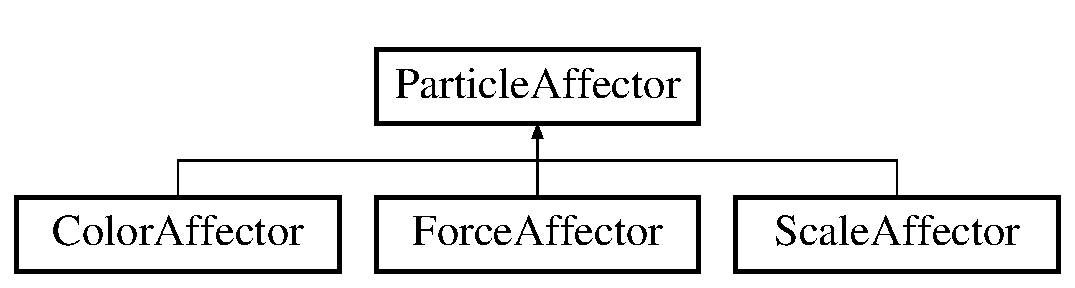
\includegraphics[height=2.000000cm]{class_particle_affector}
\end{center}
\end{figure}
\subsection*{Public Member Functions}
\begin{DoxyCompactItemize}
\item 
\mbox{\Hypertarget{class_particle_affector_aa4331fb5ef547b3dd57067b2d2c6a5d9}\label{class_particle_affector_aa4331fb5ef547b3dd57067b2d2c6a5d9}} 
virtual void \mbox{\hyperlink{class_particle_affector_aa4331fb5ef547b3dd57067b2d2c6a5d9}{affect\+Particle\+Update}} (\mbox{\hyperlink{class_particle_object}{Particle\+Object}} $\ast$particle)=0
\begin{DoxyCompactList}\small\item\em interpolate the values based on the current life of the particle \end{DoxyCompactList}\end{DoxyCompactItemize}


The documentation for this class was generated from the following file\+:\begin{DoxyCompactItemize}
\item 
F\+P\+S Counter/Particle\+Affector.\+h\end{DoxyCompactItemize}

\hypertarget{class_particle_object}{}\section{Particle\+Object Class Reference}
\label{class_particle_object}\index{Particle\+Object@{Particle\+Object}}
Inheritance diagram for Particle\+Object\+:\begin{figure}[H]
\begin{center}
\leavevmode
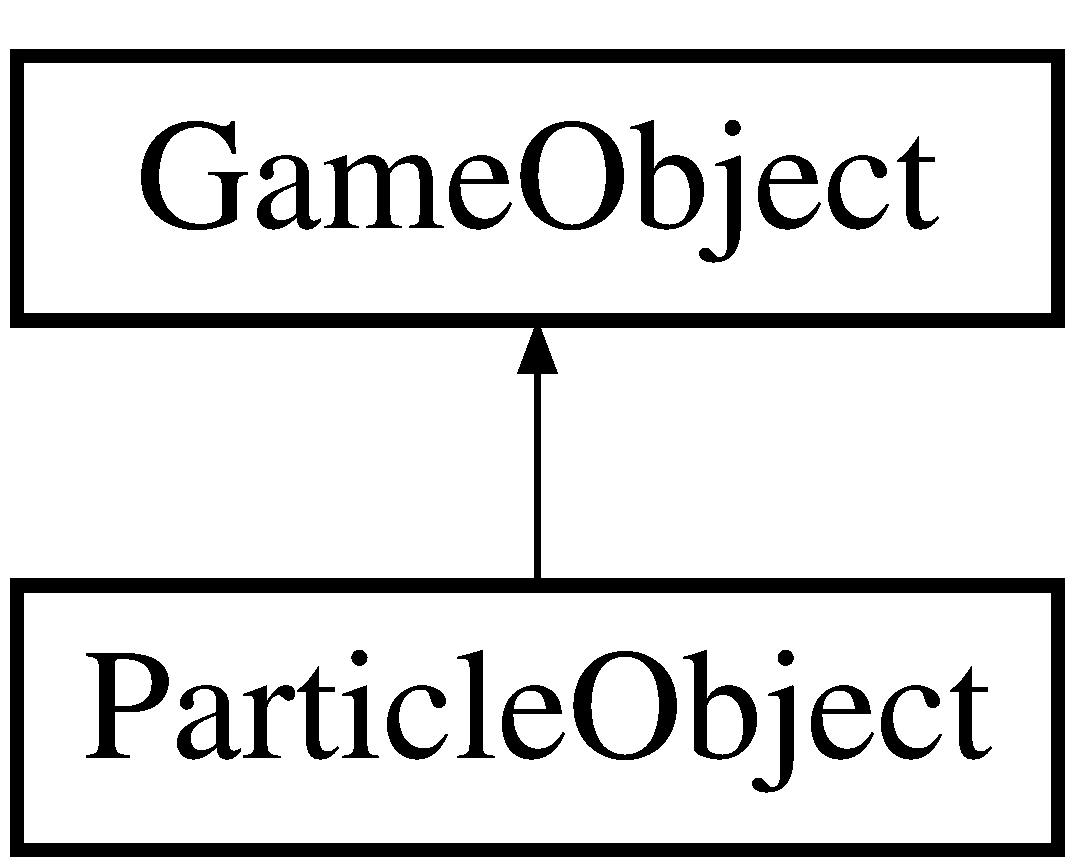
\includegraphics[height=2.000000cm]{class_particle_object}
\end{center}
\end{figure}
\subsection*{Public Member Functions}
\begin{DoxyCompactItemize}
\item 
\mbox{\Hypertarget{class_particle_object_a6071a8df79065cfc8cbb02898b09706c}\label{class_particle_object_a6071a8df79065cfc8cbb02898b09706c}} 
\mbox{\hyperlink{class_particle_object_a6071a8df79065cfc8cbb02898b09706c}{Particle\+Object}} ()
\begin{DoxyCompactList}\small\item\em Default Constructor. \end{DoxyCompactList}\item 
\mbox{\Hypertarget{class_particle_object_a68676885f0457e0737568192fa9e15f7}\label{class_particle_object_a68676885f0457e0737568192fa9e15f7}} 
\mbox{\hyperlink{class_particle_object_a68676885f0457e0737568192fa9e15f7}{Particle\+Object}} (\mbox{\hyperlink{class_sprite}{Sprite}} $\ast$sprite)
\begin{DoxyCompactList}\small\item\em Constructor. \end{DoxyCompactList}\item 
\mbox{\Hypertarget{class_particle_object_a26e462b7b677c7afdb21029c1c994887}\label{class_particle_object_a26e462b7b677c7afdb21029c1c994887}} 
void {\bfseries update} ()
\item 
\mbox{\Hypertarget{class_particle_object_ae64d28c67cc907a4c0d7b8cd369e2900}\label{class_particle_object_ae64d28c67cc907a4c0d7b8cd369e2900}} 
float \mbox{\hyperlink{class_particle_object_ae64d28c67cc907a4c0d7b8cd369e2900}{Get\+Life}} ()
\begin{DoxyCompactList}\small\item\em Returns the current remaining life on particle object. \end{DoxyCompactList}\item 
\mbox{\Hypertarget{class_particle_object_af1f1263c291261bcec3a65de1606ffaa}\label{class_particle_object_af1f1263c291261bcec3a65de1606ffaa}} 
float \mbox{\hyperlink{class_particle_object_af1f1263c291261bcec3a65de1606ffaa}{Get\+Life\+Passed}} ()
\begin{DoxyCompactList}\small\item\em Returns the time passed for particle object. \end{DoxyCompactList}\item 
\mbox{\Hypertarget{class_particle_object_a47bfcd02614d825170995695cda65173}\label{class_particle_object_a47bfcd02614d825170995695cda65173}} 
float \mbox{\hyperlink{class_particle_object_a47bfcd02614d825170995695cda65173}{Get\+Init\+Life}} ()
\begin{DoxyCompactList}\small\item\em Returns the initial lifetime of particle object. \end{DoxyCompactList}\item 
\mbox{\Hypertarget{class_particle_object_aac0db7533558c053544874257c1e2084}\label{class_particle_object_aac0db7533558c053544874257c1e2084}} 
void \mbox{\hyperlink{class_particle_object_aac0db7533558c053544874257c1e2084}{Set\+Acceleration}} (\mbox{\hyperlink{class_vector3}{Vector3}} acceleration)
\begin{DoxyCompactList}\small\item\em Set the acceleration of particle object. \end{DoxyCompactList}\item 
\mbox{\Hypertarget{class_particle_object_af778cead64627866bbd7a8a3140e42d3}\label{class_particle_object_af778cead64627866bbd7a8a3140e42d3}} 
void \mbox{\hyperlink{class_particle_object_af778cead64627866bbd7a8a3140e42d3}{Set\+Max\+Velocity}} (float magnitude)
\begin{DoxyCompactList}\small\item\em Set the maximum velocity (magnitude) of particle object. Setting this to 0 would remove any limit. \end{DoxyCompactList}\item 
\mbox{\Hypertarget{class_particle_object_a4903b5643e136f02384eba6a38dfd624}\label{class_particle_object_a4903b5643e136f02384eba6a38dfd624}} 
void \mbox{\hyperlink{class_particle_object_a4903b5643e136f02384eba6a38dfd624}{Set\+Life}} (float life)
\begin{DoxyCompactList}\small\item\em Set the lifetime of particle object in frames. \end{DoxyCompactList}\end{DoxyCompactItemize}
\subsection*{Additional Inherited Members}


The documentation for this class was generated from the following files\+:\begin{DoxyCompactItemize}
\item 
F\+P\+S Counter/Particle\+Object.\+h\item 
F\+P\+S Counter/Particle\+Object.\+cpp\end{DoxyCompactItemize}

\hypertarget{class_particlesystem}{}\section{Particlesystem Class Reference}
\label{class_particlesystem}\index{Particlesystem@{Particlesystem}}
\subsection*{Public Member Functions}
\begin{DoxyCompactItemize}
\item 
\mbox{\Hypertarget{class_particlesystem_a269b86f194b90cac301a302cc729bf25}\label{class_particlesystem_a269b86f194b90cac301a302cc729bf25}} 
{\bfseries Particlesystem} (\mbox{\hyperlink{class_sprite}{Sprite}} $\ast$sprite)
\item 
\mbox{\Hypertarget{class_particlesystem_a1bad47872a55fa997546ecbdeeff23be}\label{class_particlesystem_a1bad47872a55fa997546ecbdeeff23be}} 
\mbox{\hyperlink{class_particlesystem_a1bad47872a55fa997546ecbdeeff23be}{Particlesystem}} (\mbox{\hyperlink{class_sprite}{Sprite}} $\ast$sprite, float emission\+Rate, float emission\+Level, int particle\+Count, float max\+Life=0.\+0f)
\begin{DoxyCompactList}\small\item\em Constructor for the Particle System. \end{DoxyCompactList}\item 
\mbox{\Hypertarget{class_particlesystem_a7cb7b6f716c5dc5247db9641380dbaad}\label{class_particlesystem_a7cb7b6f716c5dc5247db9641380dbaad}} 
void \mbox{\hyperlink{class_particlesystem_a7cb7b6f716c5dc5247db9641380dbaad}{add\+Affector}} (\mbox{\hyperlink{class_particle_affector}{Particle\+Affector}} $\ast$affector)
\begin{DoxyCompactList}\small\item\em Add a particle affector into the particle system. \end{DoxyCompactList}\item 
\mbox{\Hypertarget{class_particlesystem_acb511af57e48902ce229ba363d8bf4f4}\label{class_particlesystem_acb511af57e48902ce229ba363d8bf4f4}} 
void \mbox{\hyperlink{class_particlesystem_acb511af57e48902ce229ba363d8bf4f4}{Set\+Pos}} (\mbox{\hyperlink{class_vector3}{Vector3}} location)
\begin{DoxyCompactList}\small\item\em Set the location for particle system. \end{DoxyCompactList}\item 
\mbox{\Hypertarget{class_particlesystem_ad5434b31db421a80b5d5a4f385aedc02}\label{class_particlesystem_ad5434b31db421a80b5d5a4f385aedc02}} 
void \mbox{\hyperlink{class_particlesystem_ad5434b31db421a80b5d5a4f385aedc02}{Set\+Particle\+Life}} (float life)
\begin{DoxyCompactList}\small\item\em Set the maximum life of particle object. \end{DoxyCompactList}\item 
\mbox{\Hypertarget{class_particlesystem_ae8ba8b205313d289d3104556fc671f42}\label{class_particlesystem_ae8ba8b205313d289d3104556fc671f42}} 
void \mbox{\hyperlink{class_particlesystem_ae8ba8b205313d289d3104556fc671f42}{update}} (void)
\begin{DoxyCompactList}\small\item\em Updates the particle system, called every frame. \end{DoxyCompactList}\item 
\mbox{\Hypertarget{class_particlesystem_ab483ce19ea6bfd24408de8f325459732}\label{class_particlesystem_ab483ce19ea6bfd24408de8f325459732}} 
void {\bfseries draw} (void)
\end{DoxyCompactItemize}


The documentation for this class was generated from the following files\+:\begin{DoxyCompactItemize}
\item 
F\+P\+S Counter/Particle\+Systemh.\+h\item 
F\+P\+S Counter/Particle\+Systemh.\+cpp\end{DoxyCompactItemize}

\hypertarget{class_random}{}\section{Random Class Reference}
\label{class_random}\index{Random@{Random}}
\subsection*{Static Public Member Functions}
\begin{DoxyCompactItemize}
\item 
\mbox{\Hypertarget{class_random_ac281663a3c59056bda0b2242735c2d6f}\label{class_random_ac281663a3c59056bda0b2242735c2d6f}} 
static float \mbox{\hyperlink{class_random_ac281663a3c59056bda0b2242735c2d6f}{rand\+\_\+0\+\_\+1}} (void)
\begin{DoxyCompactList}\small\item\em return value from 0.\+0 -\/ 1.\+0 \end{DoxyCompactList}\item 
\mbox{\Hypertarget{class_random_ac12473be88fe8388e54b892c2994b652}\label{class_random_ac12473be88fe8388e54b892c2994b652}} 
static float \mbox{\hyperlink{class_random_ac12473be88fe8388e54b892c2994b652}{randf}} (float min, float max)
\begin{DoxyCompactList}\small\item\em return int value in between min, max (including min and max itself) \end{DoxyCompactList}\item 
\mbox{\Hypertarget{class_random_a73a1fc971dc0e46eae612e0b02924b63}\label{class_random_a73a1fc971dc0e46eae612e0b02924b63}} 
static float \mbox{\hyperlink{class_random_a73a1fc971dc0e46eae612e0b02924b63}{randi}} (int min, int max)
\begin{DoxyCompactList}\small\item\em return float value in between min, max (including min and max itself) \end{DoxyCompactList}\item 
\mbox{\Hypertarget{class_random_aea2f96bdfb95f2aabba9a94c0f9b40f1}\label{class_random_aea2f96bdfb95f2aabba9a94c0f9b40f1}} 
static void \mbox{\hyperlink{class_random_aea2f96bdfb95f2aabba9a94c0f9b40f1}{Set\+Seed}} (int seed)
\begin{DoxyCompactList}\small\item\em Set the seed of the randomizer, call this function before performing any randomization. \end{DoxyCompactList}\end{DoxyCompactItemize}


The documentation for this class was generated from the following files\+:\begin{DoxyCompactItemize}
\item 
F\+P\+S Counter/Random.\+h\item 
F\+P\+S Counter/Random.\+cpp\end{DoxyCompactItemize}

\hypertarget{class_scale_affector}{}\section{Scale\+Affector Class Reference}
\label{class_scale_affector}\index{Scale\+Affector@{Scale\+Affector}}


Affector that changes particle size over time.  




{\ttfamily \#include $<$Particle\+Affector.\+h$>$}

Inheritance diagram for Scale\+Affector\+:\begin{figure}[H]
\begin{center}
\leavevmode
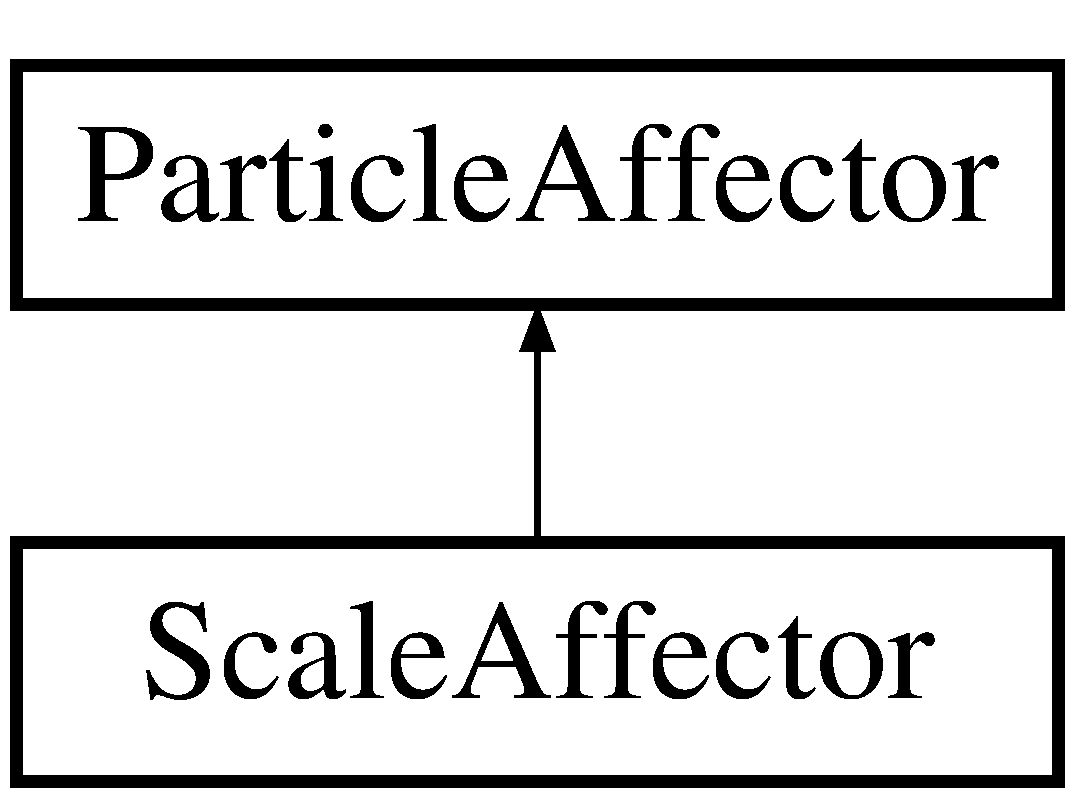
\includegraphics[height=2.000000cm]{class_scale_affector}
\end{center}
\end{figure}
\subsection*{Public Member Functions}
\begin{DoxyCompactItemize}
\item 
\mbox{\Hypertarget{class_scale_affector_a28d6f4d64b67735347eae8c8d05da2e2}\label{class_scale_affector_a28d6f4d64b67735347eae8c8d05da2e2}} 
\mbox{\hyperlink{class_scale_affector_a28d6f4d64b67735347eae8c8d05da2e2}{Scale\+Affector}} (float start\+Scale, float end\+Scale)
\begin{DoxyCompactList}\small\item\em Constructor. start\+Scale \+: the scale of particle starts with. end\+Scale \+: the scale the particle would interpolate towards. \end{DoxyCompactList}\item 
\mbox{\Hypertarget{class_scale_affector_aed5224f20a6c4c1474d202df5a192544}\label{class_scale_affector_aed5224f20a6c4c1474d202df5a192544}} 
virtual void \mbox{\hyperlink{class_scale_affector_aed5224f20a6c4c1474d202df5a192544}{affect\+Particle\+Update}} (\mbox{\hyperlink{class_particle_object}{Particle\+Object}} $\ast$particle)
\begin{DoxyCompactList}\small\item\em interpolate the values based on the current life of the particle \end{DoxyCompactList}\end{DoxyCompactItemize}


\subsection{Detailed Description}
Affector that changes particle size over time. 

The documentation for this class was generated from the following files\+:\begin{DoxyCompactItemize}
\item 
F\+P\+S Counter/Particle\+Affector.\+h\item 
F\+P\+S Counter/Particle\+Affector.\+cpp\end{DoxyCompactItemize}

\hypertarget{class_sprite}{}\section{Sprite Class Reference}
\label{class_sprite}\index{Sprite@{Sprite}}
\subsection*{Public Member Functions}
\begin{DoxyCompactItemize}
\item 
\mbox{\Hypertarget{class_sprite_a7f8f0cbc76b11c16860fbda7f1e23ef1}\label{class_sprite_a7f8f0cbc76b11c16860fbda7f1e23ef1}} 
{\bfseries Sprite} (const std\+::string \&file)
\item 
\mbox{\Hypertarget{class_sprite_aa93521985ef2c64b860a5d81dd90c23a}\label{class_sprite_aa93521985ef2c64b860a5d81dd90c23a}} 
void {\bfseries draw} (float x, float y, float scale=1.\+0f, float rotation=0.\+0f, Color color=\+Color\+::white, enum\+Blend blendmode=enum\+Blend\+::alpha)
\end{DoxyCompactItemize}
\subsection*{Static Public Attributes}
\begin{DoxyCompactItemize}
\item 
\mbox{\Hypertarget{class_sprite_a4828d83bfc97792c9a3b9c337817adaf}\label{class_sprite_a4828d83bfc97792c9a3b9c337817adaf}} 
static \mbox{\hyperlink{class_color}{Color}} {\bfseries color}
\end{DoxyCompactItemize}


The documentation for this class was generated from the following files\+:\begin{DoxyCompactItemize}
\item 
F\+P\+S Counter/Sprite.\+h\item 
F\+P\+S Counter/Sprite.\+cpp\end{DoxyCompactItemize}

\hypertarget{structucvector}{}\section{ucvector Struct Reference}
\label{structucvector}\index{ucvector@{ucvector}}
\subsection*{Public Attributes}
\begin{DoxyCompactItemize}
\item 
\mbox{\Hypertarget{structucvector_ace794c5713208c5a20f21762cd87c919}\label{structucvector_ace794c5713208c5a20f21762cd87c919}} 
unsigned char $\ast$ {\bfseries data}
\item 
\mbox{\Hypertarget{structucvector_a27c99c34de0c5b3ca0c242d402c69499}\label{structucvector_a27c99c34de0c5b3ca0c242d402c69499}} 
size\+\_\+t {\bfseries size}
\item 
\mbox{\Hypertarget{structucvector_a235168baac13f0c78bd3e309dc170f90}\label{structucvector_a235168baac13f0c78bd3e309dc170f90}} 
size\+\_\+t {\bfseries allocsize}
\end{DoxyCompactItemize}


The documentation for this struct was generated from the following file\+:\begin{DoxyCompactItemize}
\item 
F\+P\+S Counter/lodepng.\+cpp\end{DoxyCompactItemize}

\hypertarget{structuivector}{}\section{uivector Struct Reference}
\label{structuivector}\index{uivector@{uivector}}
\subsection*{Public Attributes}
\begin{DoxyCompactItemize}
\item 
\mbox{\Hypertarget{structuivector_a427d761df4bb4f0f19b4a973fc224c78}\label{structuivector_a427d761df4bb4f0f19b4a973fc224c78}} 
unsigned $\ast$ {\bfseries data}
\item 
\mbox{\Hypertarget{structuivector_aa999025945f0c93d0461192475ae2720}\label{structuivector_aa999025945f0c93d0461192475ae2720}} 
size\+\_\+t {\bfseries size}
\item 
\mbox{\Hypertarget{structuivector_aac0395a9ad397ae7a28219561ab49ffa}\label{structuivector_aac0395a9ad397ae7a28219561ab49ffa}} 
size\+\_\+t {\bfseries allocsize}
\end{DoxyCompactItemize}


The documentation for this struct was generated from the following file\+:\begin{DoxyCompactItemize}
\item 
F\+P\+S Counter/lodepng.\+cpp\end{DoxyCompactItemize}

\hypertarget{class_vector3}{}\section{Vector3 Class Reference}
\label{class_vector3}\index{Vector3@{Vector3}}
\subsection*{Public Member Functions}
\begin{DoxyCompactItemize}
\item 
\mbox{\Hypertarget{class_vector3_ad53e22b52babdb90d423601f72467590}\label{class_vector3_ad53e22b52babdb90d423601f72467590}} 
{\bfseries Vector3} (float x, float y, float z)
\item 
\mbox{\Hypertarget{class_vector3_a6a854b71c4f3449407b55084b8babf9d}\label{class_vector3_a6a854b71c4f3449407b55084b8babf9d}} 
\mbox{\hyperlink{class_vector3}{Vector3}} {\bfseries operator+} (\mbox{\hyperlink{class_vector3}{Vector3}} value)
\item 
\mbox{\Hypertarget{class_vector3_a991fdefb3666c676986e81e6bc6b5f4d}\label{class_vector3_a991fdefb3666c676986e81e6bc6b5f4d}} 
\mbox{\hyperlink{class_vector3}{Vector3}} {\bfseries operator-\/} (\mbox{\hyperlink{class_vector3}{Vector3}} value)
\item 
\mbox{\Hypertarget{class_vector3_a368ea66b05c77e7ff5138b3306e2f6ea}\label{class_vector3_a368ea66b05c77e7ff5138b3306e2f6ea}} 
\mbox{\hyperlink{class_vector3}{Vector3}} {\bfseries operator$\ast$} (float value)
\item 
\mbox{\Hypertarget{class_vector3_a8325f1befd63b95c74c1f758d6263f22}\label{class_vector3_a8325f1befd63b95c74c1f758d6263f22}} 
\mbox{\hyperlink{class_vector3}{Vector3}} {\bfseries operator/} (float value)
\item 
\mbox{\Hypertarget{class_vector3_ad82c10e9ea6eb6f707cd1e507f1100d2}\label{class_vector3_ad82c10e9ea6eb6f707cd1e507f1100d2}} 
\mbox{\hyperlink{class_vector3}{Vector3}} {\bfseries Cross} (const \mbox{\hyperlink{class_vector3}{Vector3}} \&vec)
\item 
\mbox{\Hypertarget{class_vector3_a8a8cb236aae8602af246f4f56495f159}\label{class_vector3_a8a8cb236aae8602af246f4f56495f159}} 
\mbox{\hyperlink{class_vector3}{Vector3}} {\bfseries Normalize} ()
\item 
\mbox{\Hypertarget{class_vector3_a96d7aba13eb550ee21bb046788290742}\label{class_vector3_a96d7aba13eb550ee21bb046788290742}} 
float {\bfseries Dot} (const \mbox{\hyperlink{class_vector3}{Vector3}} \&vec)
\item 
\mbox{\Hypertarget{class_vector3_a5721d97b9640951b58c40de1a893f966}\label{class_vector3_a5721d97b9640951b58c40de1a893f966}} 
float {\bfseries Magnitude} ()
\end{DoxyCompactItemize}
\subsection*{Public Attributes}
\begin{DoxyCompactItemize}
\item 
\mbox{\Hypertarget{class_vector3_a7e2d3237b29a2f29d7b3d8b2934e35f2}\label{class_vector3_a7e2d3237b29a2f29d7b3d8b2934e35f2}} 
float {\bfseries x}
\item 
\mbox{\Hypertarget{class_vector3_a86eb35a9fa2d5a49e7fad66a35fa9c13}\label{class_vector3_a86eb35a9fa2d5a49e7fad66a35fa9c13}} 
float {\bfseries y}
\item 
\mbox{\Hypertarget{class_vector3_aa8c9461eb24bd2c364258078811a3e9d}\label{class_vector3_aa8c9461eb24bd2c364258078811a3e9d}} 
float {\bfseries z}
\end{DoxyCompactItemize}
\subsection*{Friends}
\begin{DoxyCompactItemize}
\item 
\mbox{\Hypertarget{class_vector3_af8071adba02246ed84b6ac3e3f8d4737}\label{class_vector3_af8071adba02246ed84b6ac3e3f8d4737}} 
ostream \& {\bfseries operator$<$$<$} (ostream \&os, const \mbox{\hyperlink{class_vector3}{Vector3}} \&vec)
\end{DoxyCompactItemize}


The documentation for this class was generated from the following files\+:\begin{DoxyCompactItemize}
\item 
F\+P\+S Counter/Vector3.\+h\item 
F\+P\+S Counter/Vector3.\+cpp\end{DoxyCompactItemize}

%--- End generated contents ---

% Index
\backmatter
\newpage
\phantomsection
\clearemptydoublepage
\addcontentsline{toc}{chapter}{Index}
\printindex

\end{document}
